\documentclass[aspectratio=169]{beamer}

\usepackage[utf8]{inputenc}
\usepackage{times}
\usepackage{fontspec} % set font
\usepackage{xeCJK}
	\setCJKmainfont[AutoFakeBold=6,AutoFakeSlant=.2]{AR PL KaitiM Big5}
	\XeTeXlinebreaklocale "zh"
	\XeTeXlinebreakskip = 0pt plus 1pt

\usepackage{listings} % code
\usepackage{xcolor}
\definecolor{lightgray}{gray}{0.9}
\lstset{
	backgroundcolor=\color{lightgray},
	basicstyle=\ttfamily\small,
	showstringspaces=false,
	commentstyle=\color{red},
	keywordstyle=\color{blue},
	tabsize=2
}
\usepackage{multicol}
\usepackage{ulem} % 刪除線
\usepackage{array}
\usepackage{varwidth} % width of column of tabular

\hypersetup{colorlinks=,linkcolor=,urlcolor=blue} % href color

\usetheme{Madrid} % theorem in box

\renewcommand{\b}{\overline}
\newcommand{\C}{\mathbb{C}}
\newcommand{\E}{\Edge}
\newcommand{\N}{\mathbb{N}}
\renewcommand{\P}{\mathbb{P}}
\newcommand{\Q}{\mathbb{Q}}
\newcommand{\R}{\mathbb{R}}
\newcommand{\V}{\Vertex}
\newcommand{\Z}{\mathbb{Z}}
\newcommand{\simple}{\SetVertexSimple[MinSize=8pt]}
\newcommand{\pictures}{\includegraphics[height=4cm]}
\newcommand{\directed}{\tikzstyle{EdgeStyle}=[post]}
\newcommand{\bidirected}{\tikzstyle{EdgeStyle}=[pre and post]}
\newcommand{\degree}{^\circ}
\newcommand{\Arc}[1]{\wideparen{{#1}}}
\newcommand{\lin}{\overleftrightarrow}
\newcommand{\ray}{\overrightarrow}
\newcommand{\seg}{\overline}
\newcommand{\ang}{\angle}
\newcommand{\then}{\Rightarrow}
\newcommand{\cuz}{\because}
\newcommand{\so}{\therefore}
\newcommand{\spc}{\;\;\;\;\;\;}
\newcommand{\st}{\text{ s.t. }}
\newcommand{\claim}{\textit{Claim}}
\renewcommand{\and}{\&\&}
\renewcommand{\ll}{\longleftarrow}
\newcommand{\lr}{\longrightarrow}
\newcommand{\la}{\leftarrow}
\newcommand{\ra}{\rightarrow}
\renewcommand{\mod}[1]{\text{ (mod }#1\text )}
\newcommand{\psim}{\stackrel{+}{\sim}}
\newcommand{\msim}{\stackrel{-}{\sim}}
\newcommand{\ma}{\measuredangle}
\newcommand{\parato}{\,\|\,}
\DeclareMathOperator{\lcm}{lcm}
\DeclareMathOperator{\Spec}{Spec}
\newcommand{\tor}{ $\longrightarrow$ }
\newcommand{\p}{\mathcal{P}}
\newcommand\tab[1][0.5cm]{\hspace*{#1}}
\renewcommand{\t}[1]{\colorbox{lightgray}{\texttt{#1}}}
\newcommand{\sm}{\textasciitilde}


\newtheoremstyle{mystyle}
  {15pt}{15pt}
  {}
  {}
  {\bf}
  {.}
  {1em}
	{}

\theoremstyle{mystyle}
\newtheorem{thm}{定理}[section]
\newtheorem{thr}[thm]{引理}
\newtheorem{ex}[thm]{範例}
\newtheorem{pr}[thm]{習題}
\newtheorem{sbpr}[thm]{Subproblem}
\newtheorem{df}[thm]{定義}
\newtheorem{pp}[thm]{命題}
\newtheorem{co}[thm]{推論}
\newtheorem{for}[thm]{公式}
\newtheorem{lm}[thm]{引理}
\newtheorem{nota}[thm]{符號}
\newtheorem{cl}[thm]{Claim}
\newtheorem{rmk}[thm]{註}
\newtheorem{say}[thm]{名言}

\title{台大單車社社課 - Strava}
\author{許博翔}
\institute{}
\date{March 21, 2025}

\begin{document}
%\begin{CJK}{UTF8}{bkai}
\frame{\titlepage}
\begin{frame}{Outline}
\tableofcontents
\end{frame}
\AtBeginSection[]{
\begin{frame}{Outline}
\tableofcontents[currentsection]
\end{frame}
}
\section{簡介}

\begin{frame}{運動紀錄軟體}
\begin{itemize}
\only<1-5>{
\item 紀錄騎了什麼路線\\\pause

\includegraphics[width=3cm]{smallTaipei.png}\pause
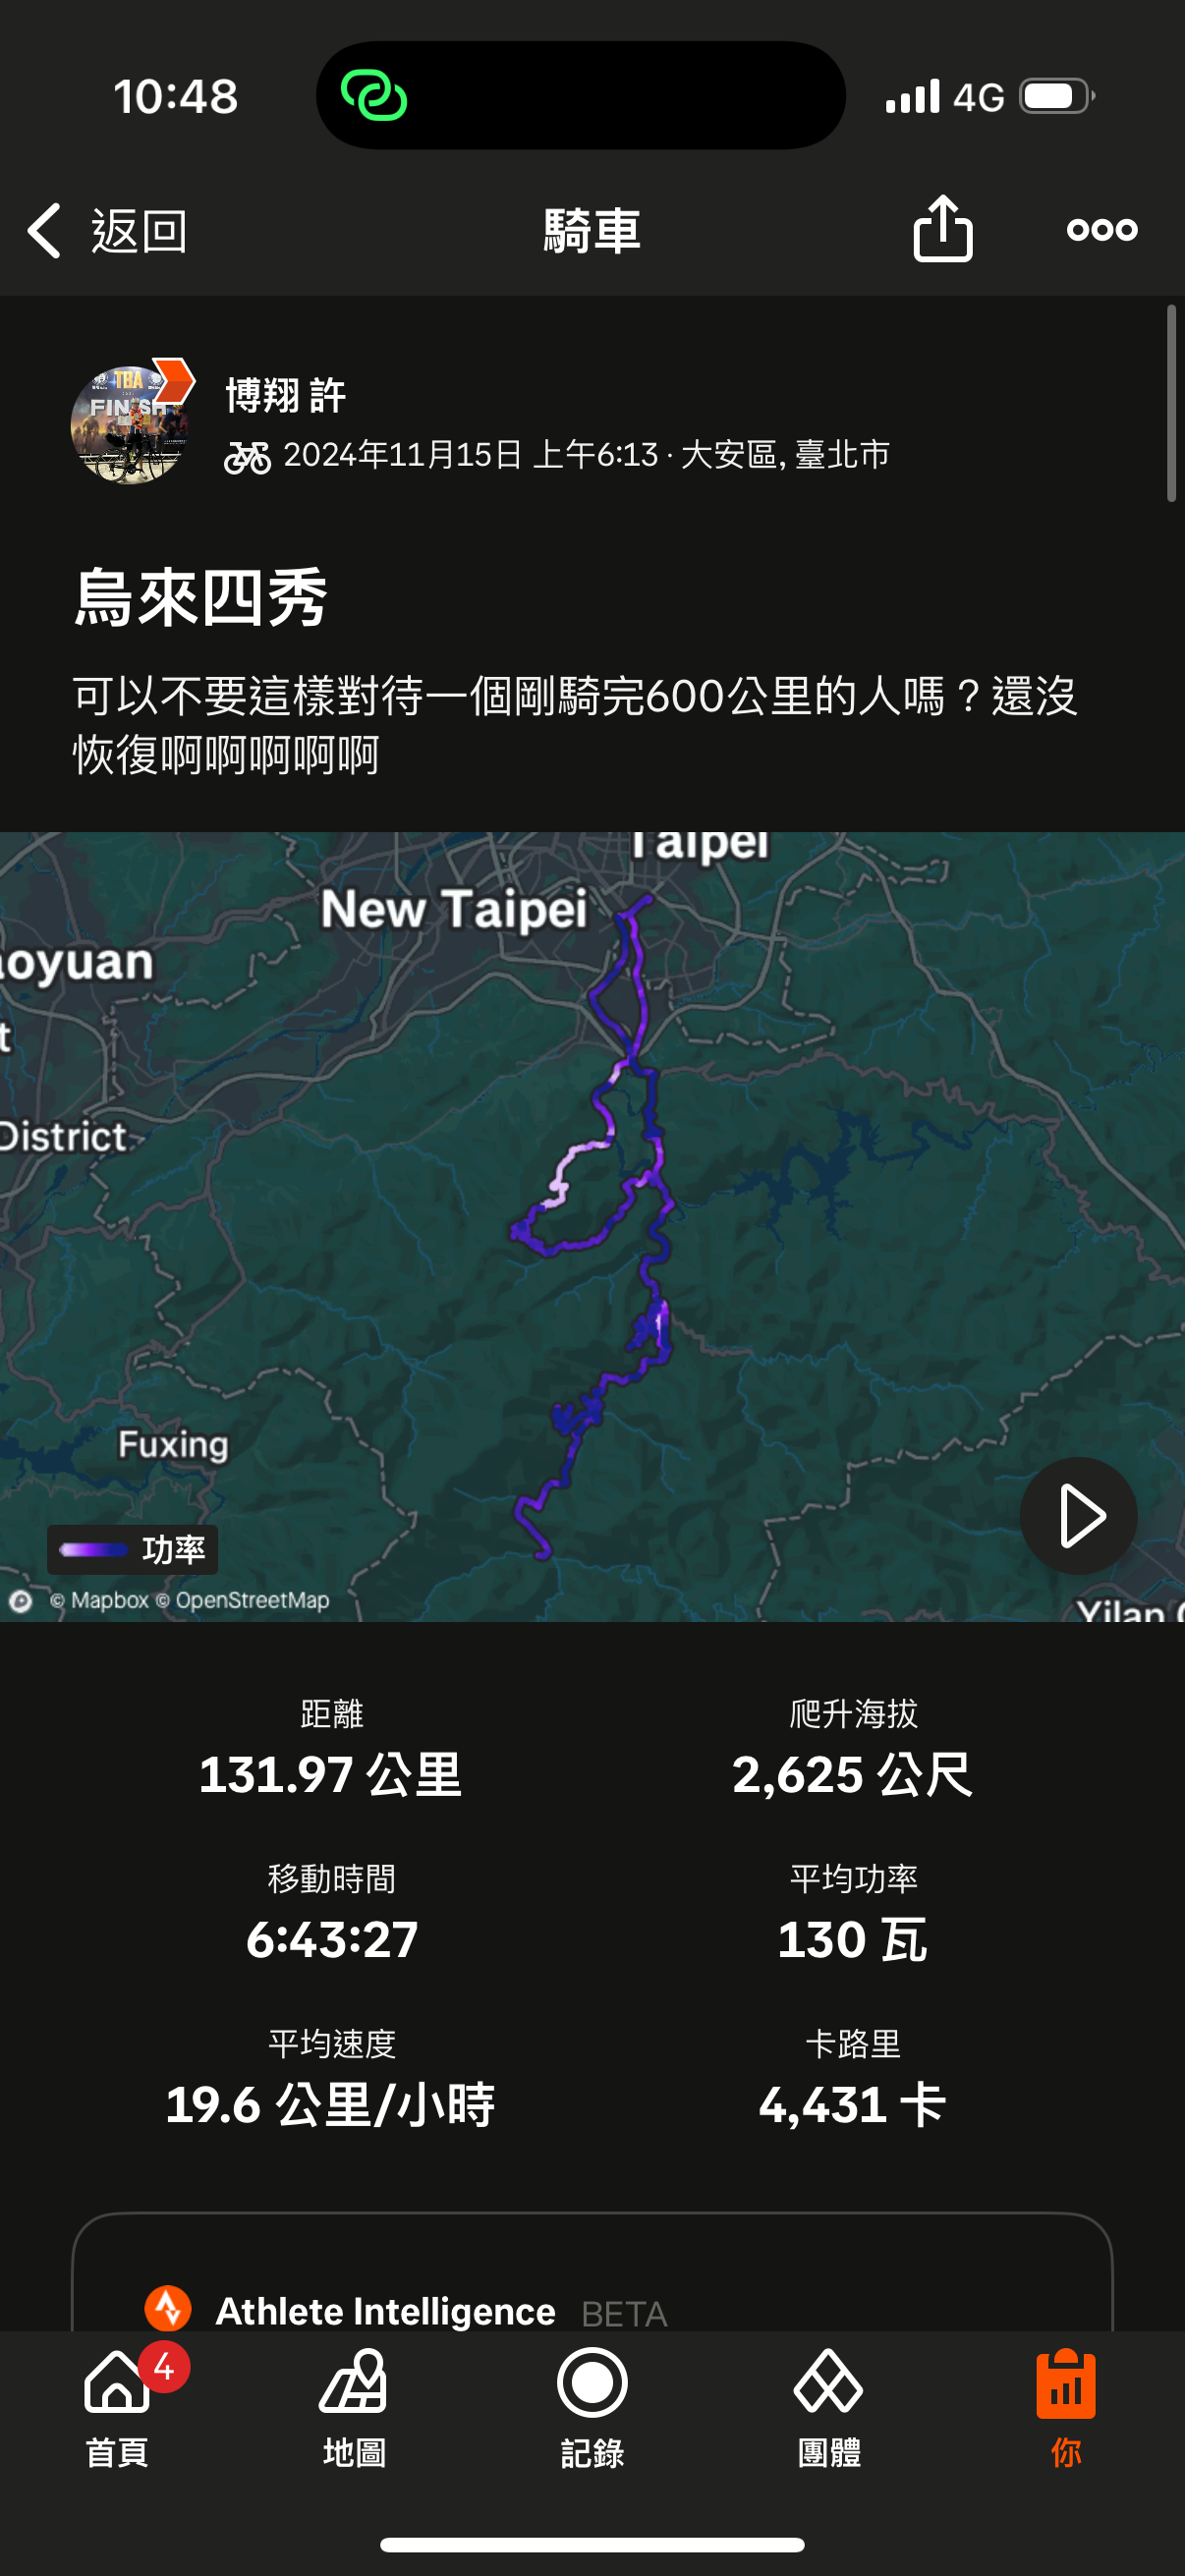
\includegraphics[width=3cm]{wulai4p.png}\pause

\includegraphics[width=3cm]{hand.png}\pause
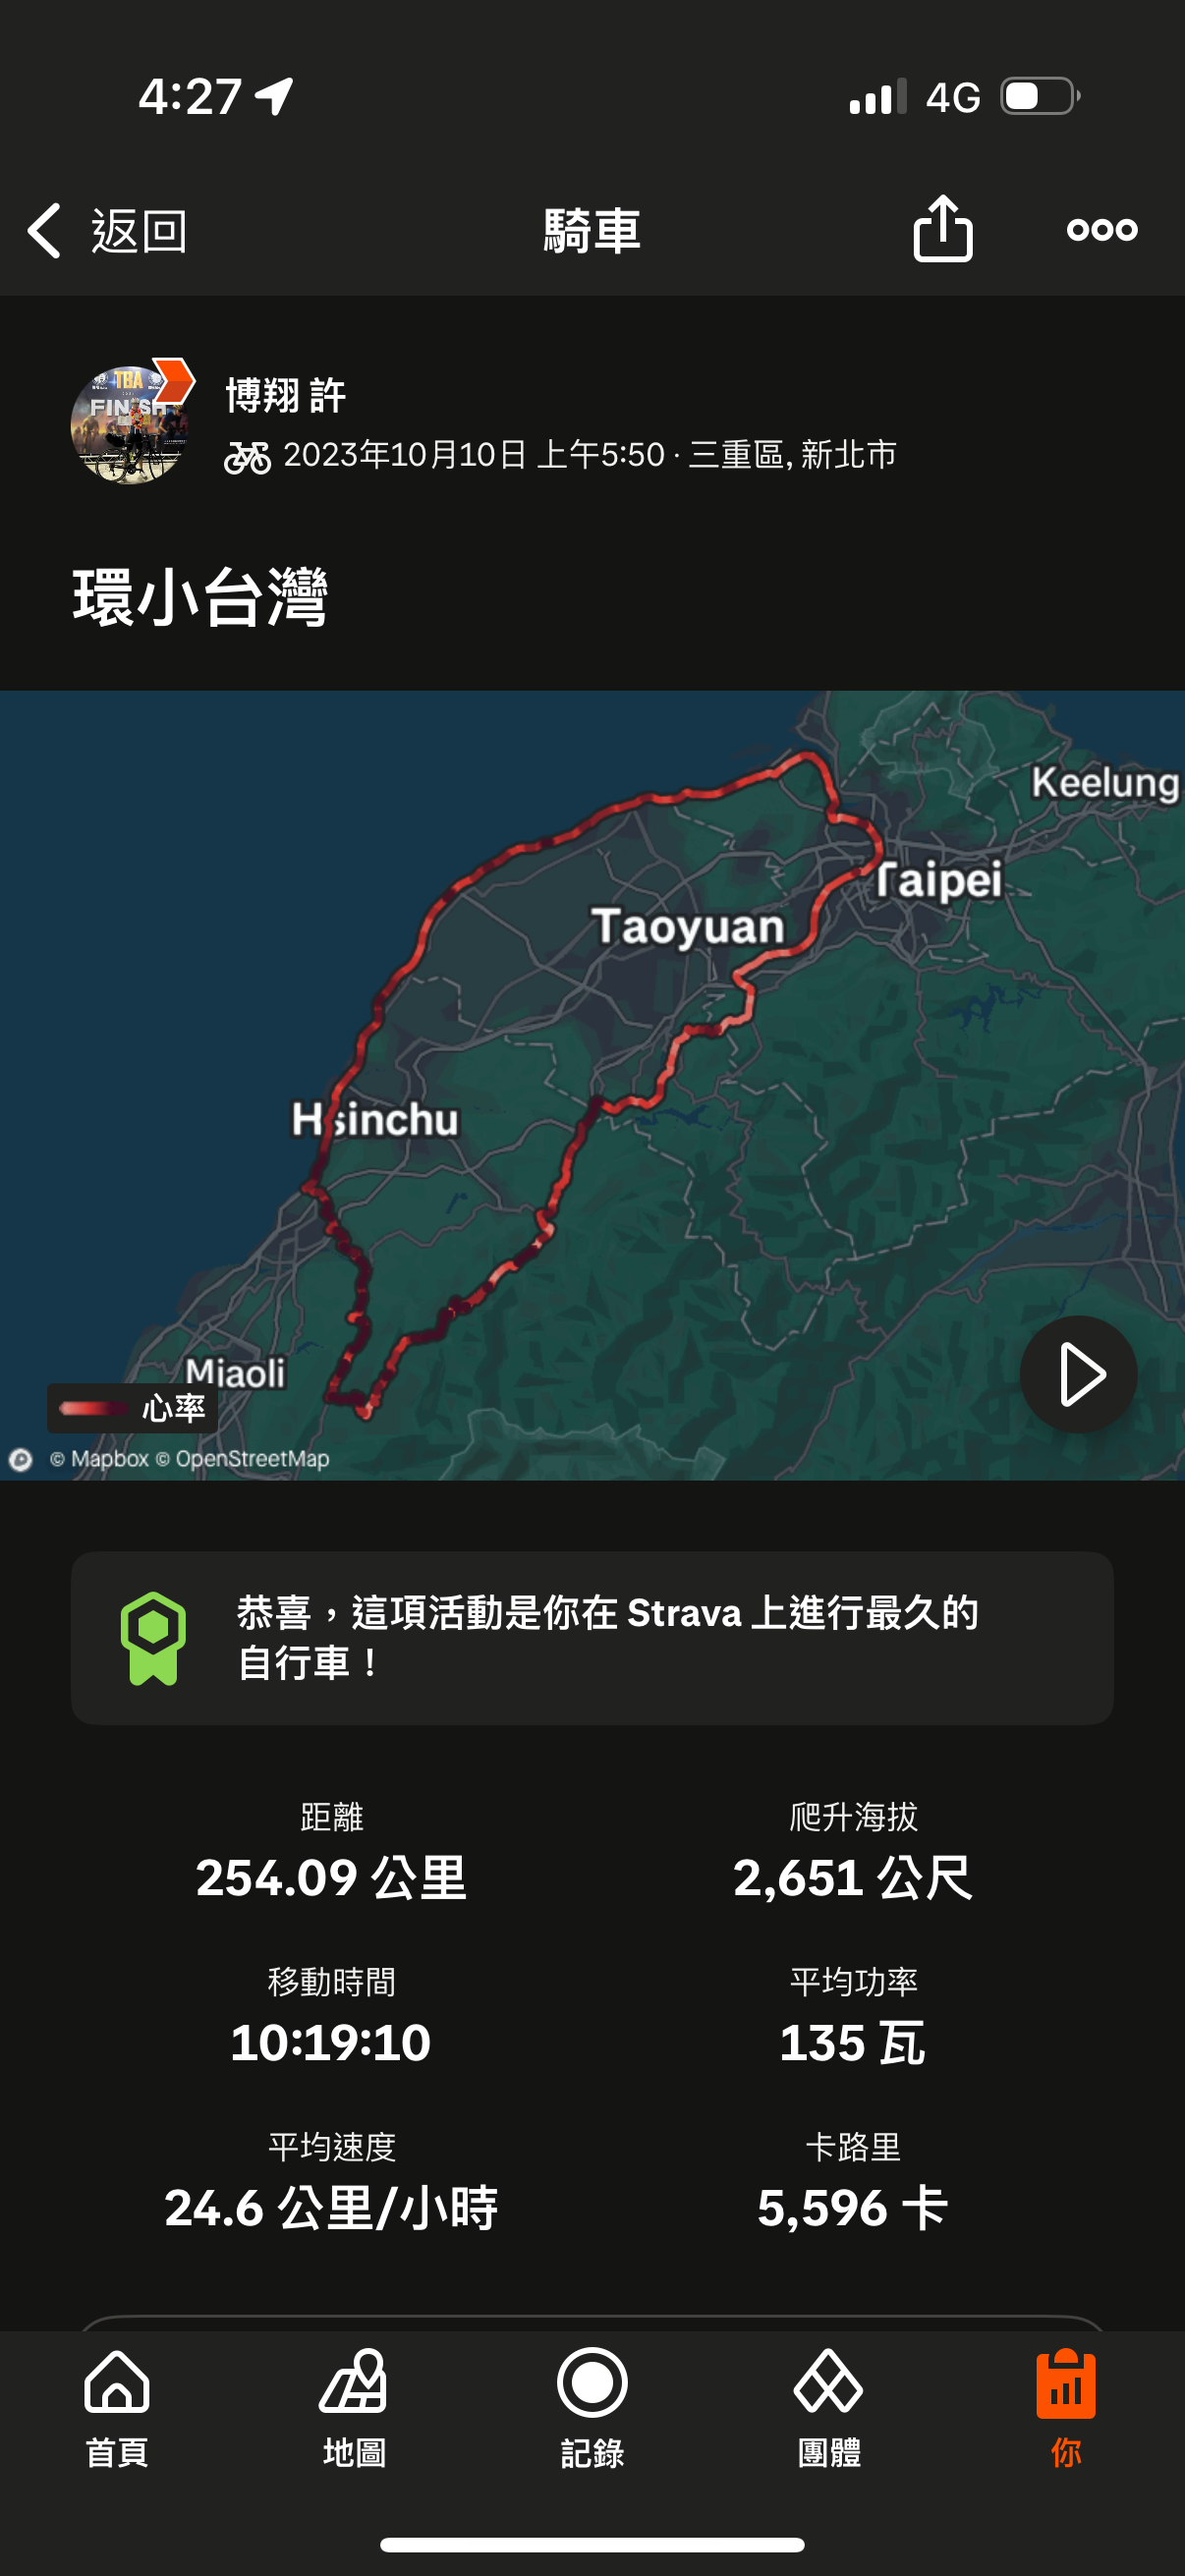
\includegraphics[width=3cm]{smallTaiwan.png}
%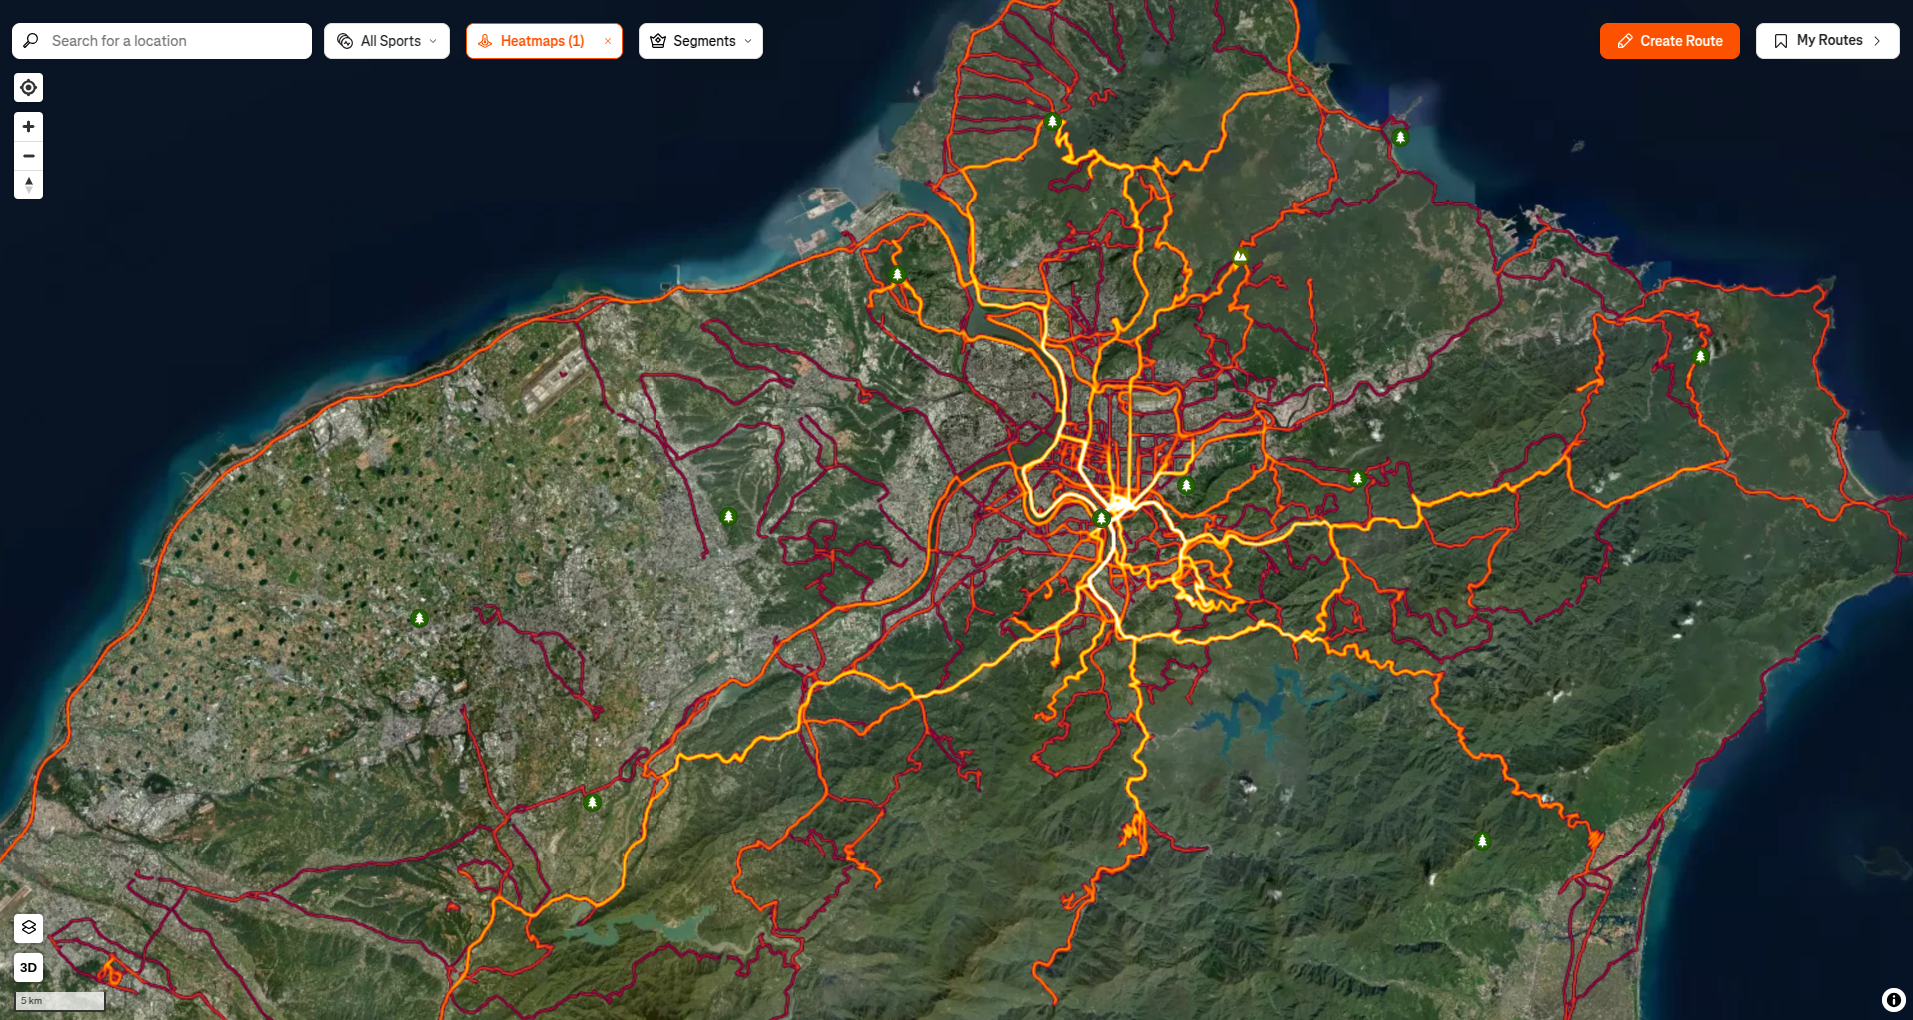
\includegraphics[width=7cm]{taipeiHeatmap.png}
%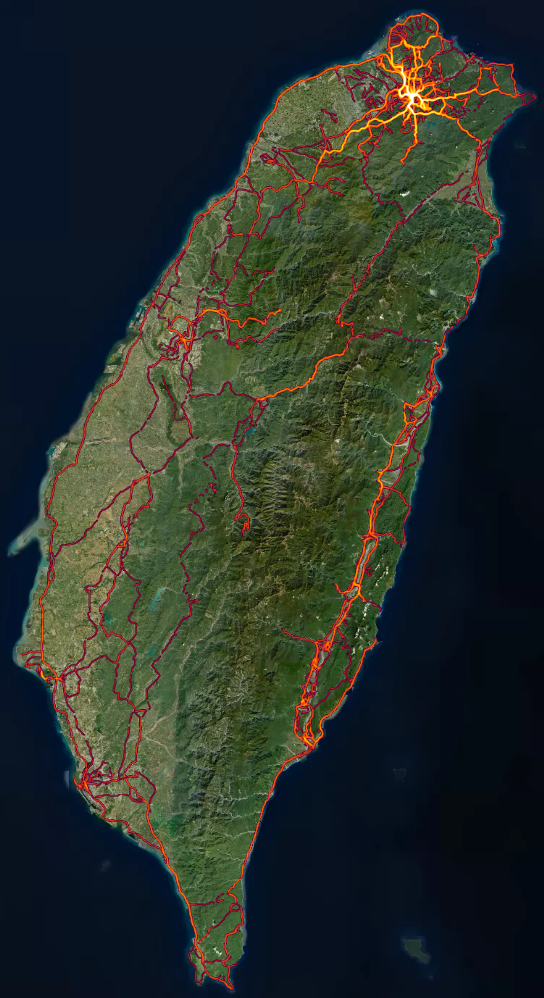
\includegraphics[width=5cm]{taiwanHeatmap.png}
}\only<6->{
\begin{multicols}{2}
\item 統計里程、爬升海拔
\item 分析騎乘的數據(速度、心率、功率等)
\item 看別人騎了什麼路線
\item 跟朋友在同個路段上競速

\includegraphics[width=3cm]{statistics2024.png}
\newpage
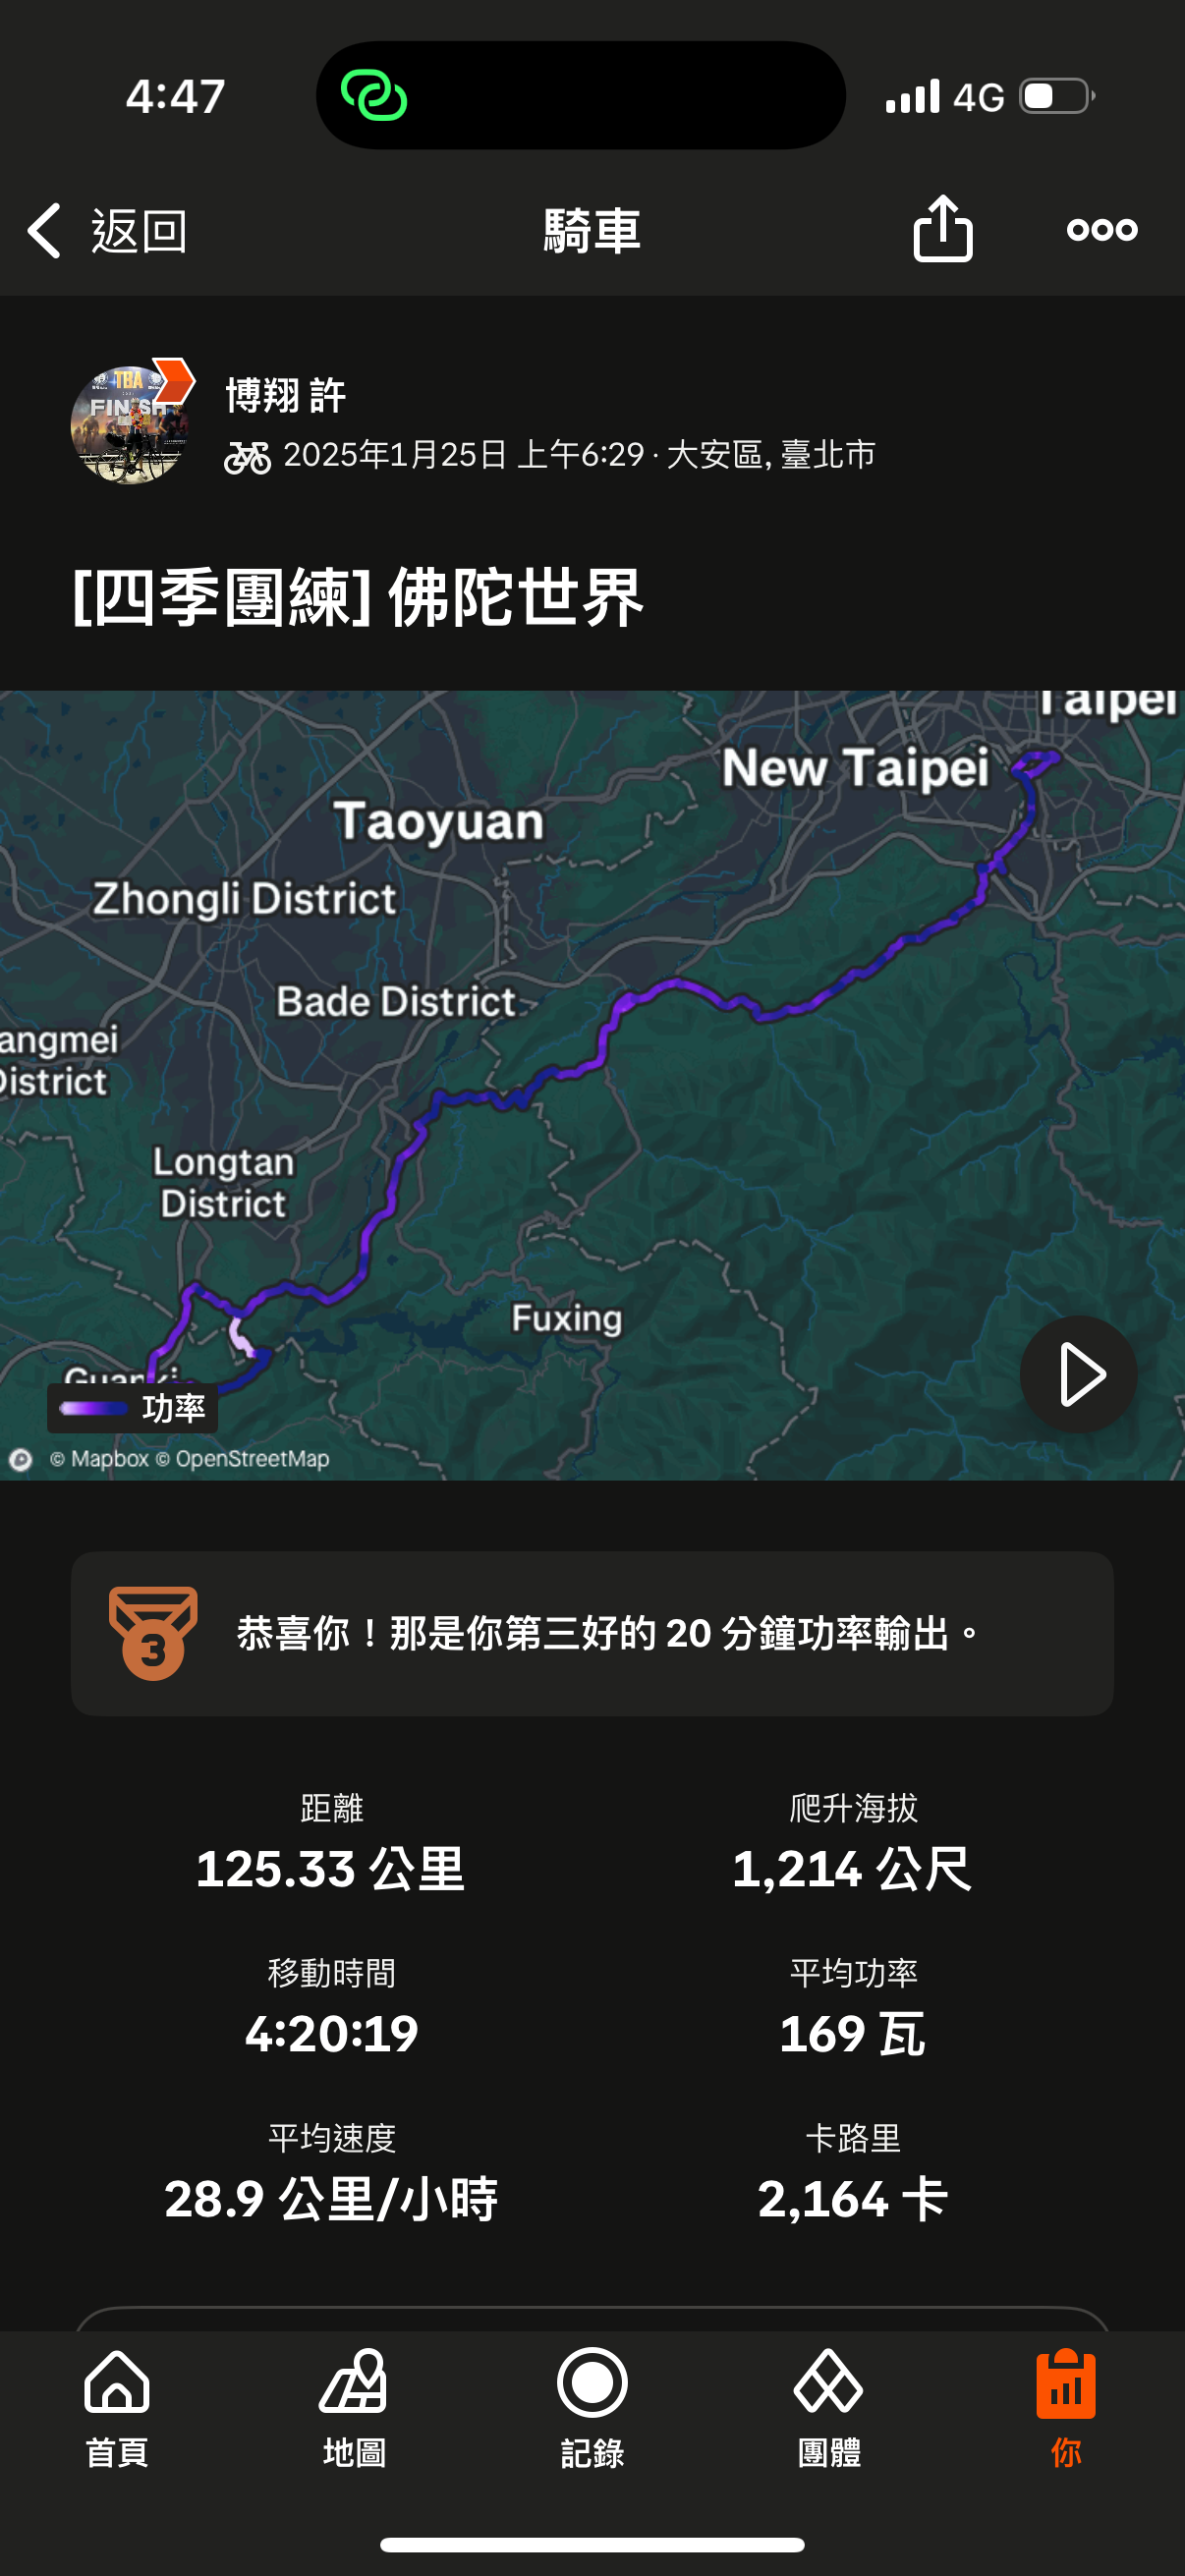
\includegraphics[width=3cm]{photoworld.png}
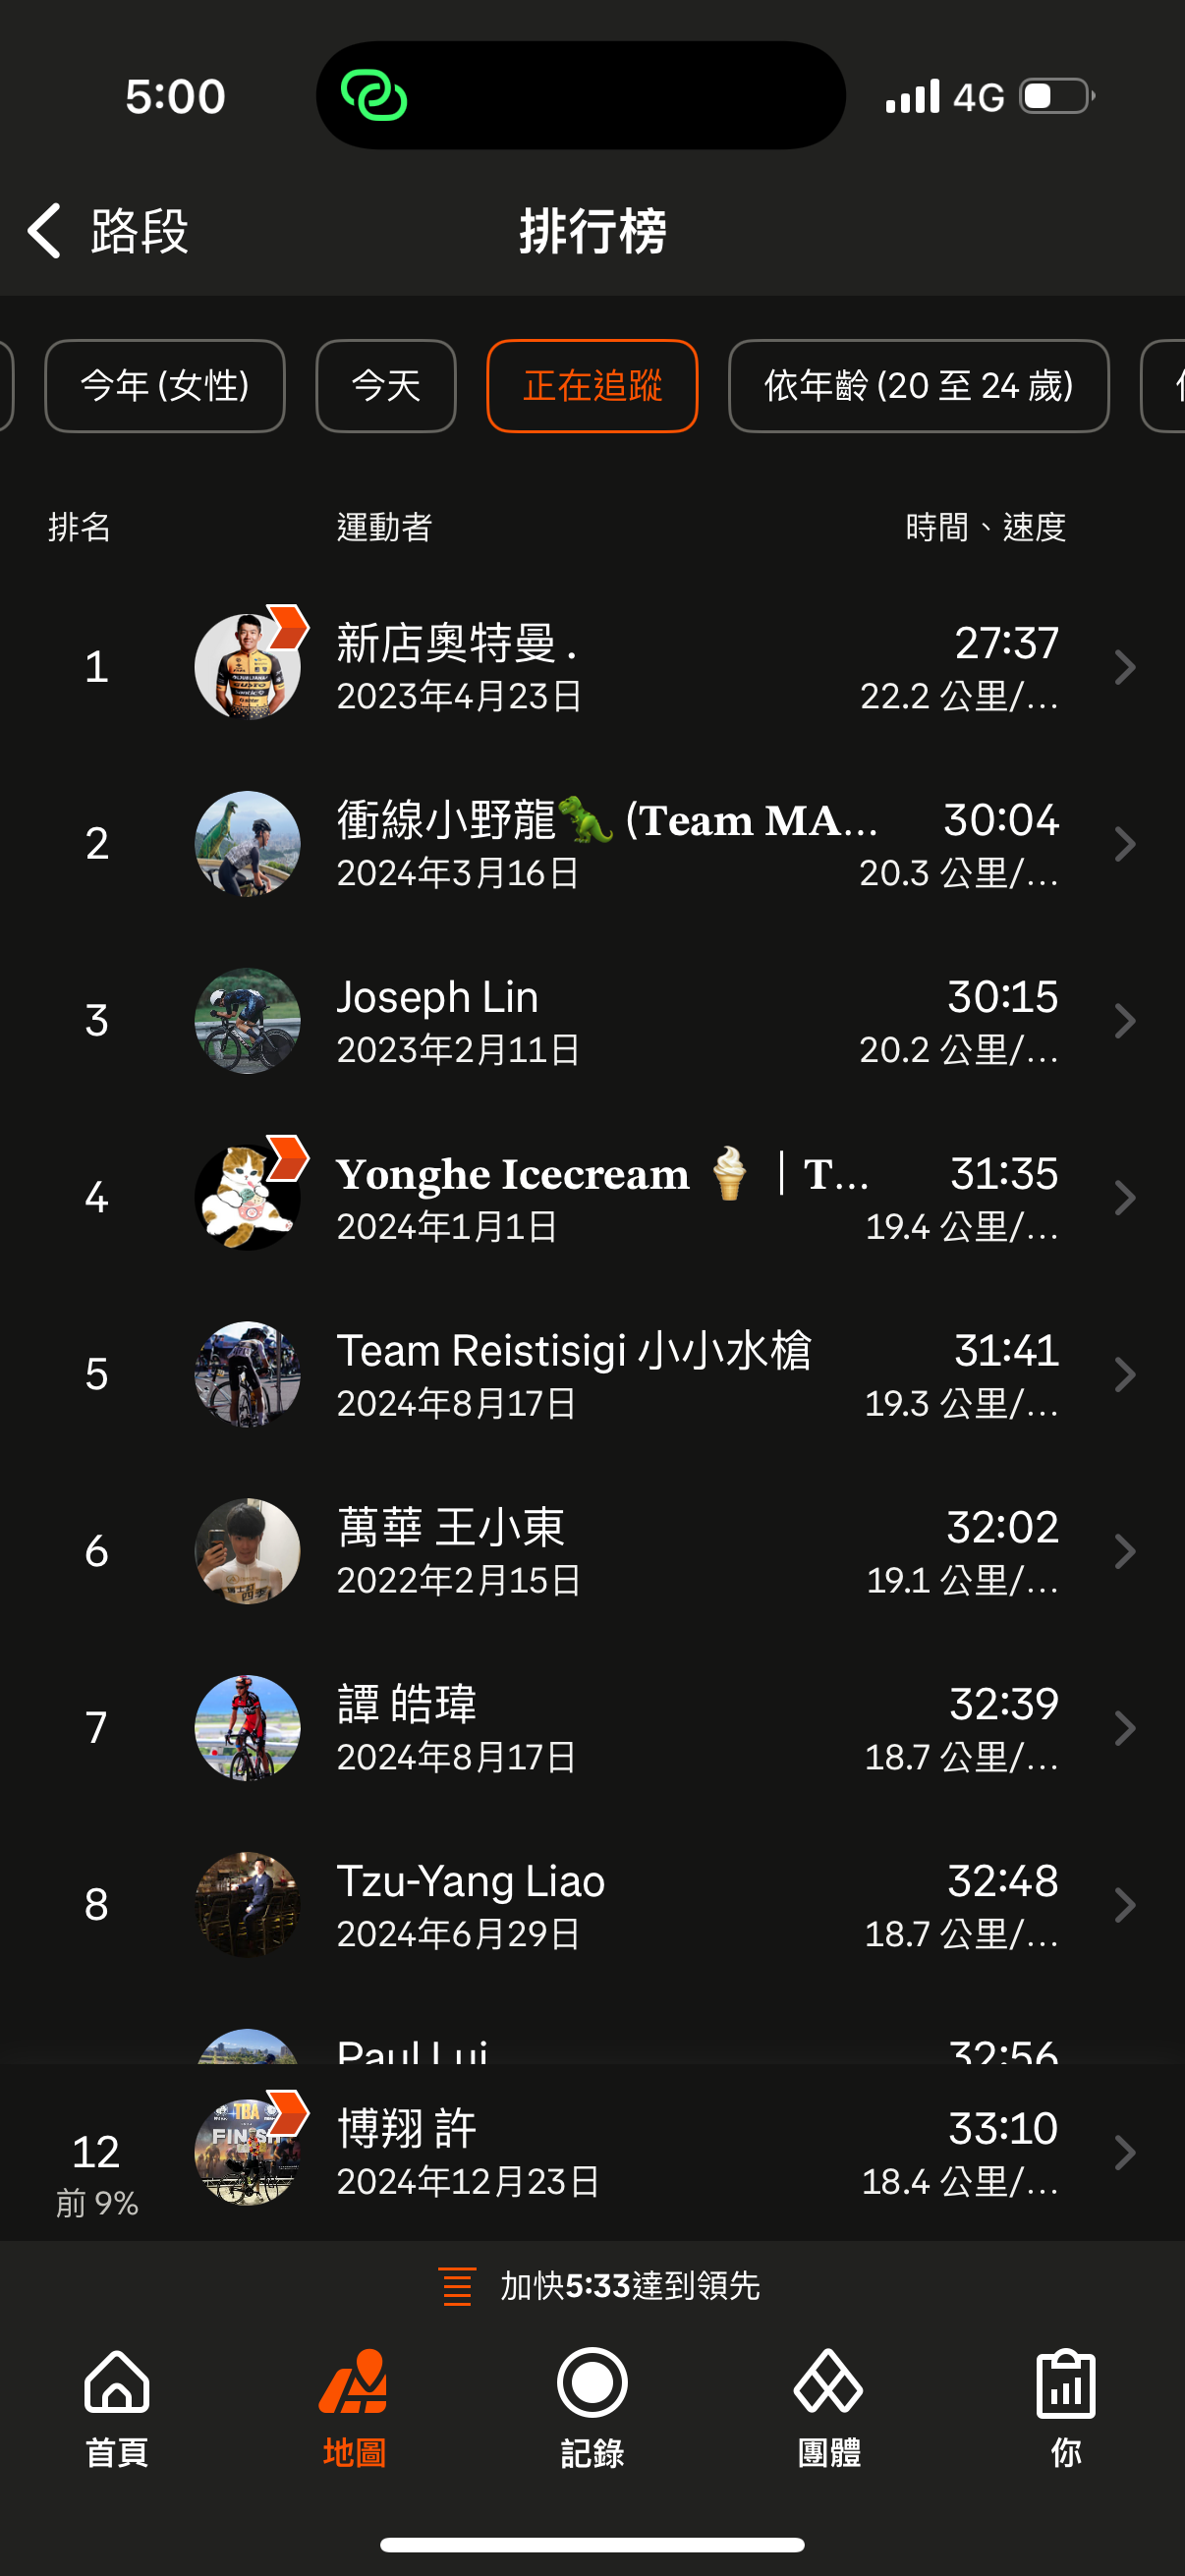
\includegraphics[width=3cm]{balakaRank.png}
\end{multicols}
}
\end{itemize}
\end{frame}

\begin{frame}{常見的運動紀錄軟體}
\begin{itemize}
\item Strava
\item Nike Run Club
\item Garmin
\item Pacer
\item Adidas Running
\item Ride with GPS
\item StepsApp
\item Walkr
\item JoiiSports
\end{itemize}
\end{frame}

\begin{frame}{Strava}
\begin{multicols}{2}
\begin{itemize}
\item 網頁:\url{https://www.strava.com}\\
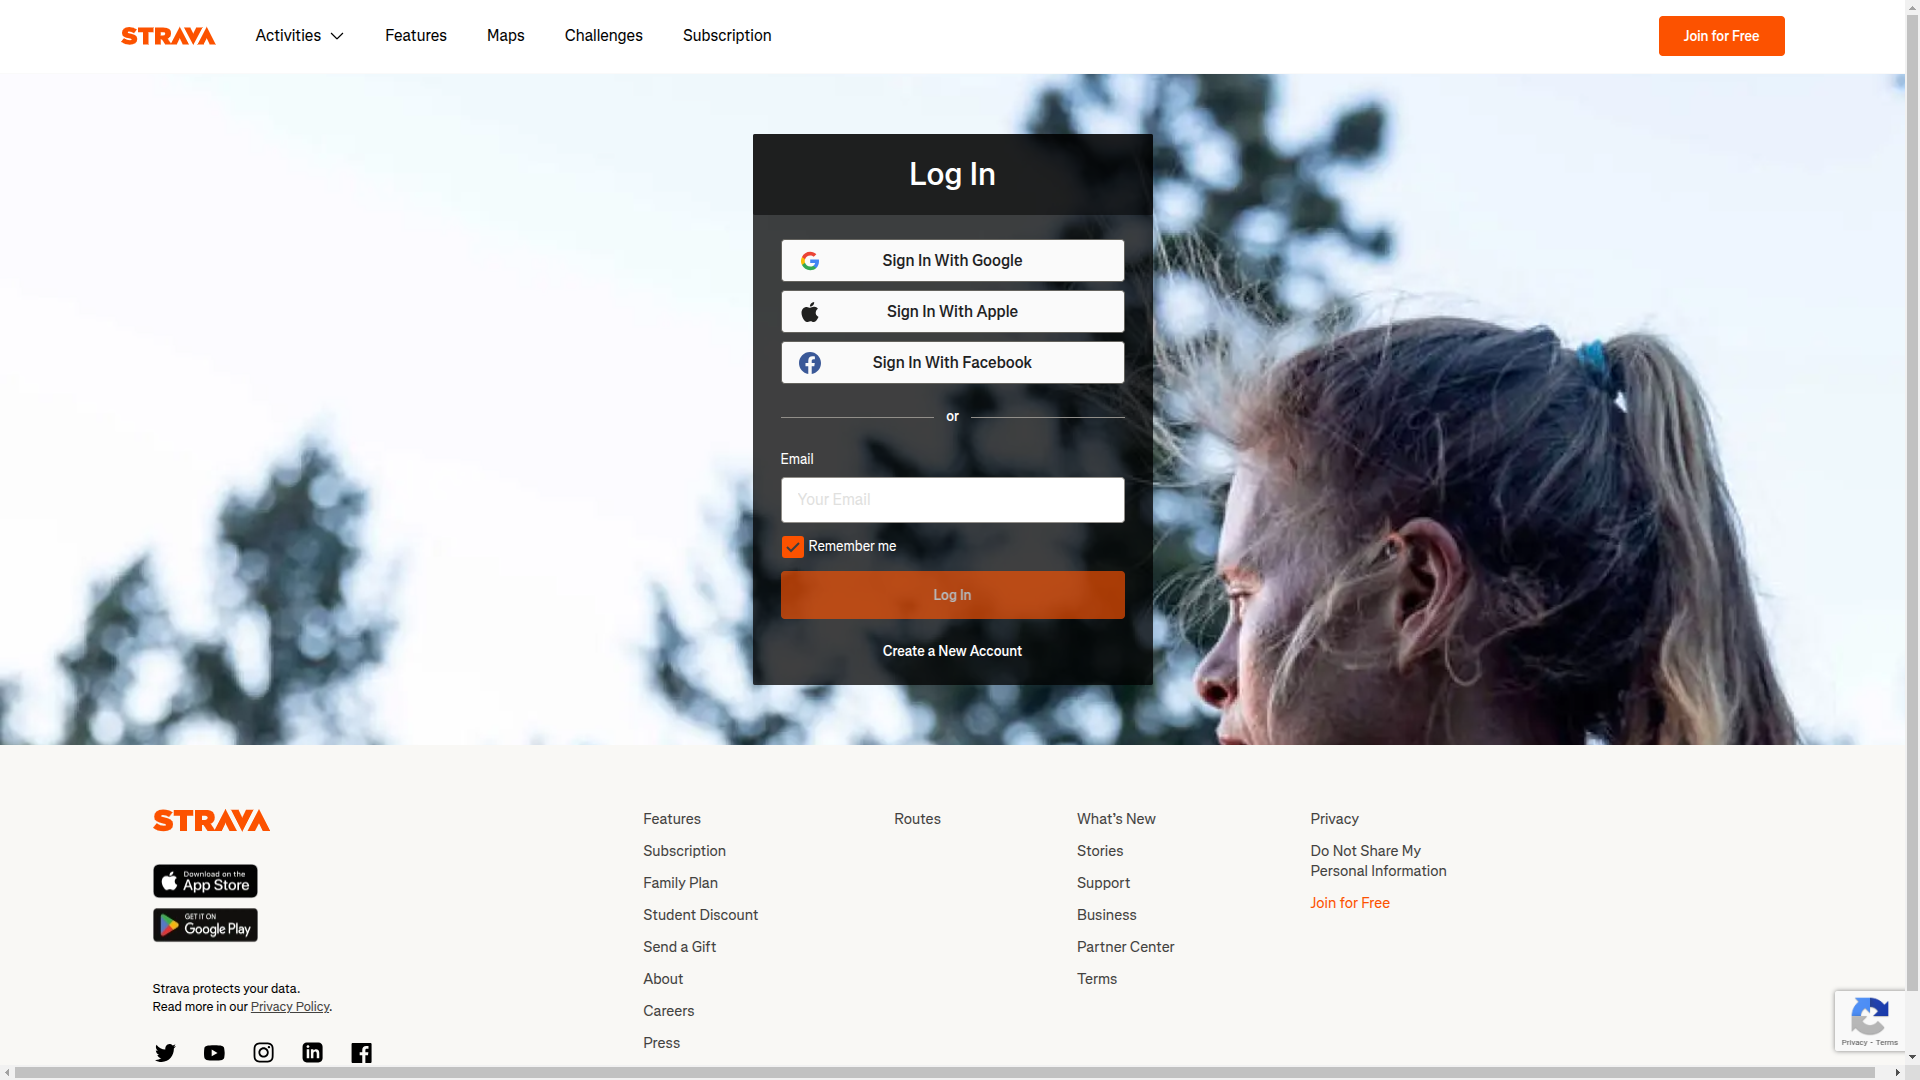
\includegraphics[width=5cm]{stravaWebsite.png}\\

\includegraphics[width=3cm]{rickroll.png}
\pause

\includegraphics[width=3cm]{QRcodeStrava.png}\pause
\newpage
\item App:搜尋「Strava」應該就會出現了\\

\includegraphics[width=5cm]{stravaApp.png}
\end{itemize}
\end{multicols}
\end{frame}

\section{基礎功能}

\begin{frame}{隱私設定}
\begin{multicols}{2}
\begin{itemize}
\item 一般權限\\
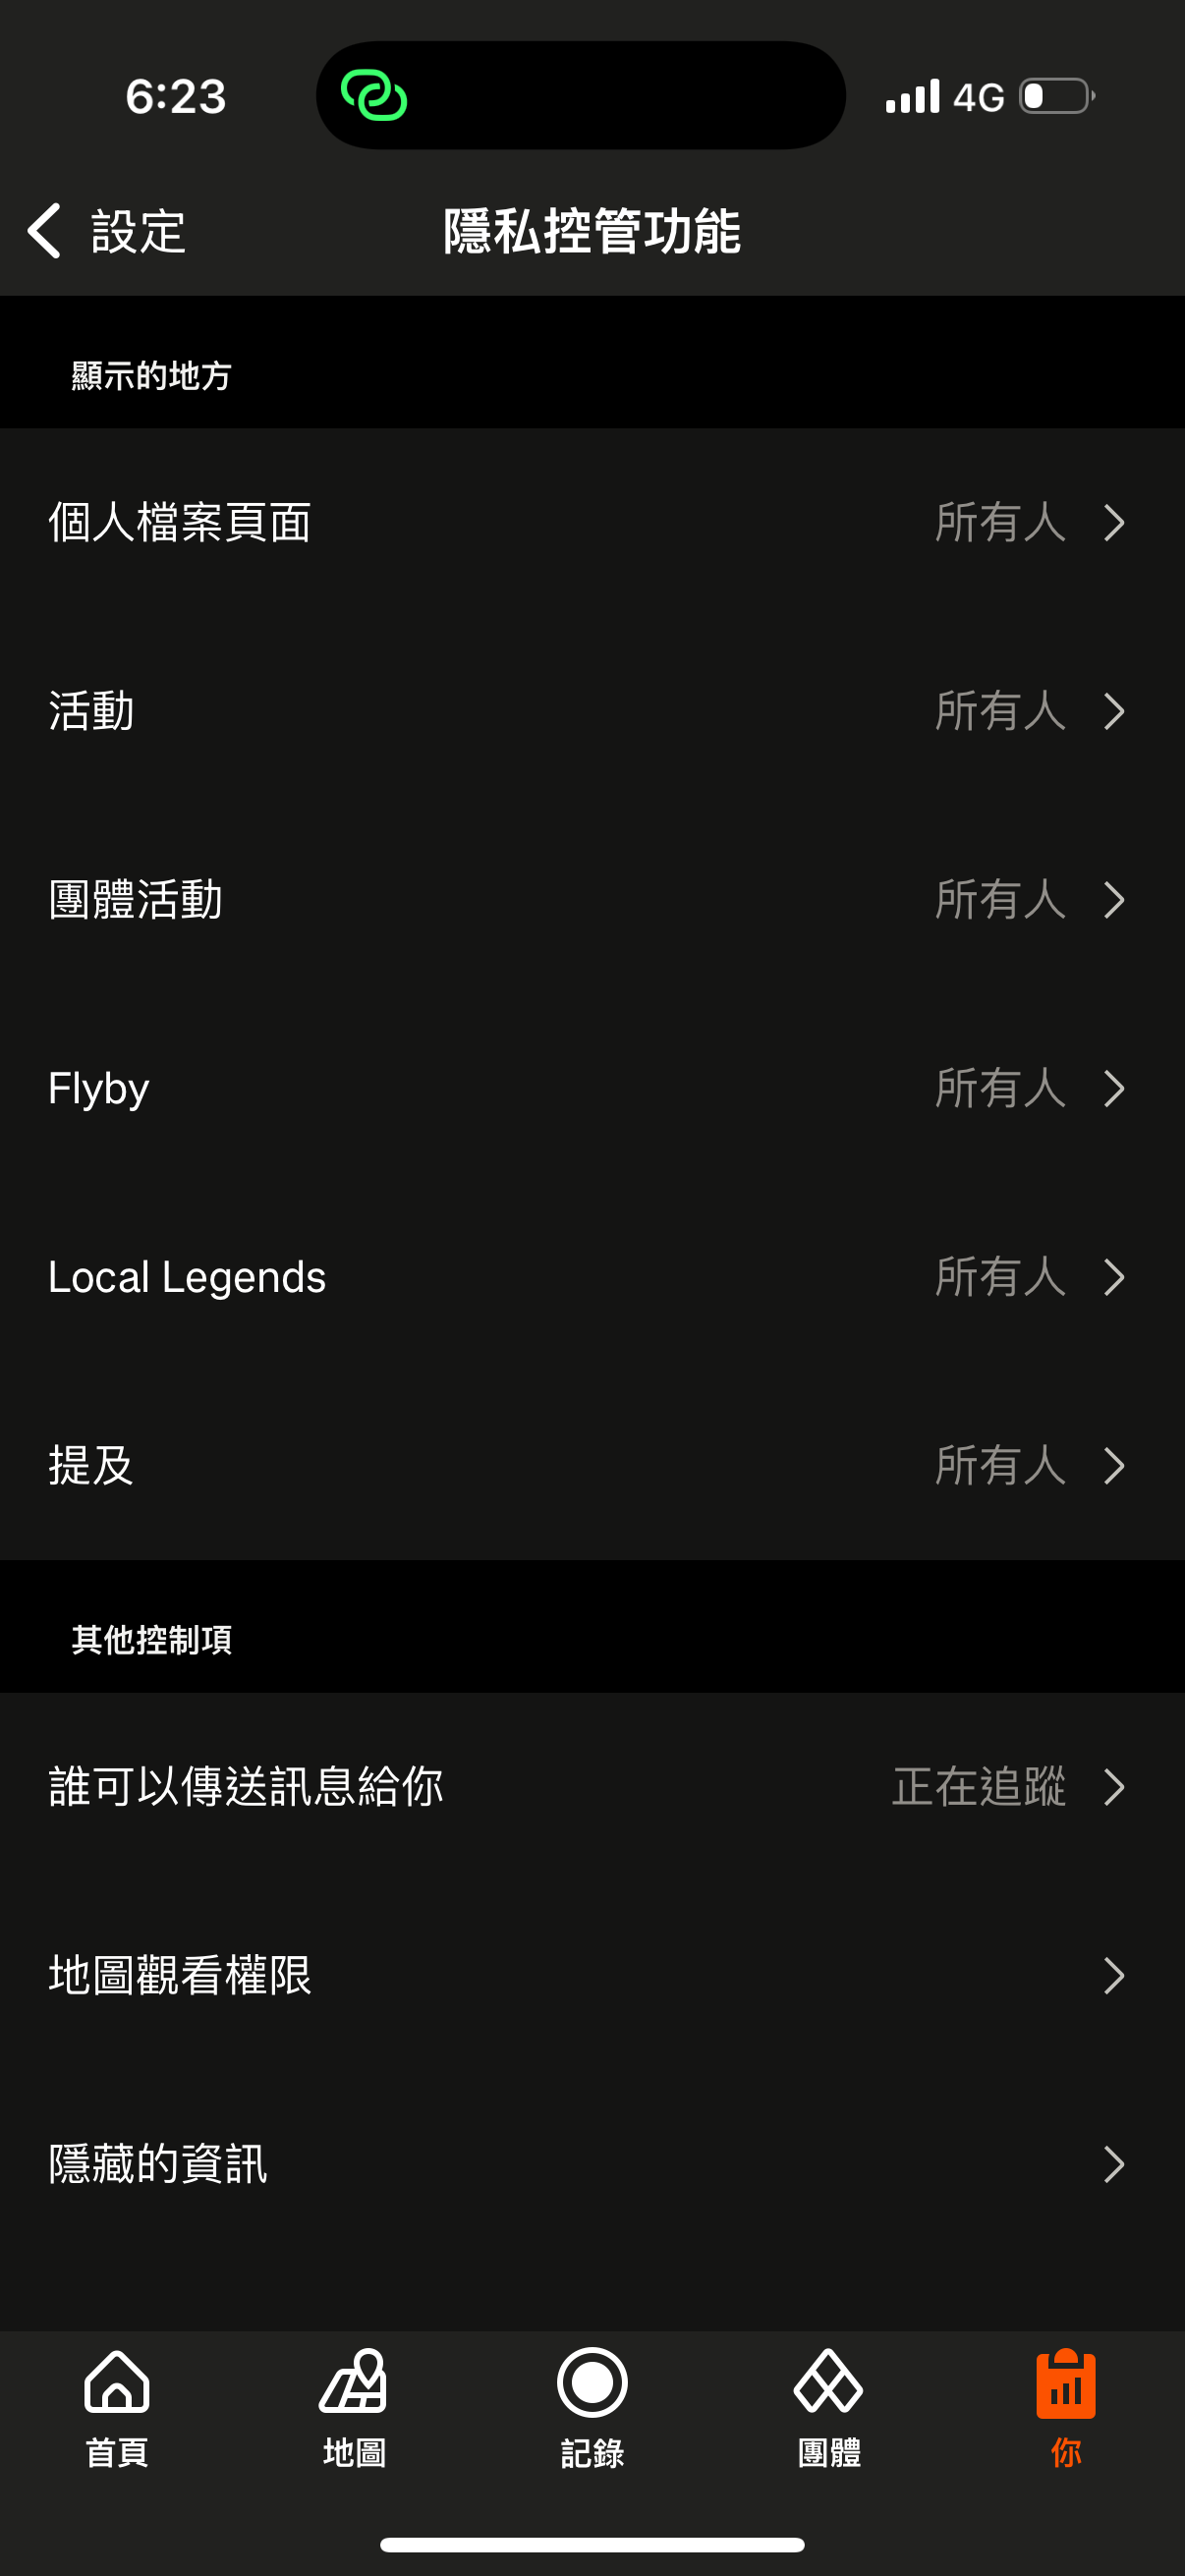
\includegraphics[width=3cm]{privacy.png}
\item 地圖觀看權限\\
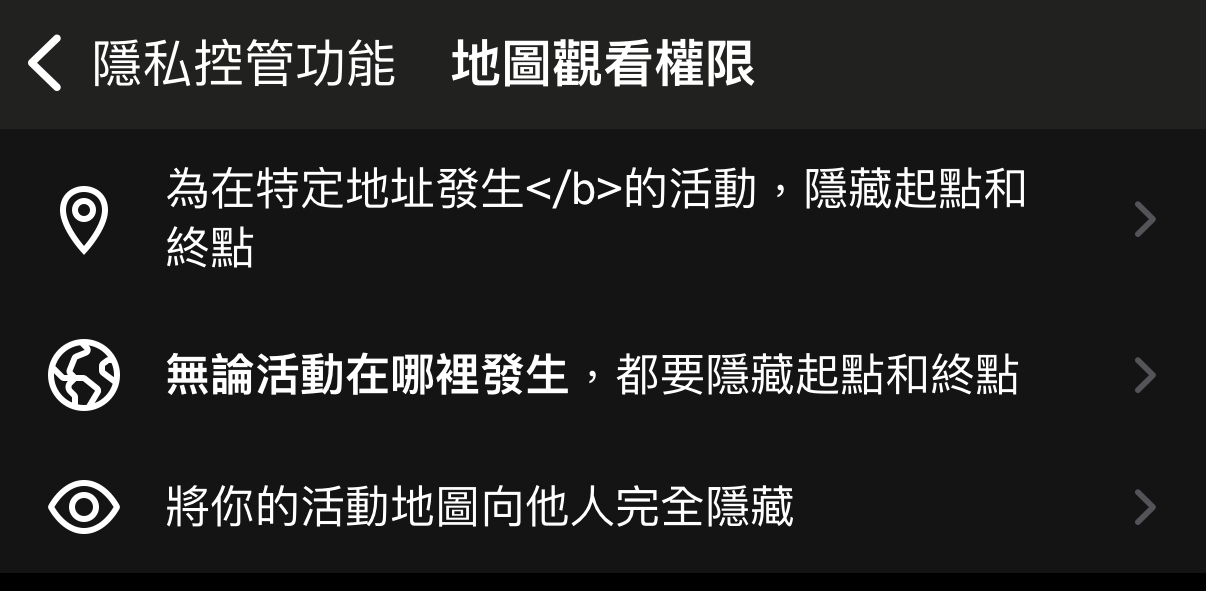
\includegraphics[width=5cm]{hideMap.png}
\end{itemize}
\end{multicols}
\end{frame}

\begin{frame}{騎車人的 Instagram}
\begin{itemize}
\only<1>{
\begin{multicols}{2}
\item 加好友\\

\includegraphics[width=3cm]{friend.png}\\
\item 也可以用搜尋的,但是要把名字放在前面姓氏放在後面搜尋
\newpage

\includegraphics[width=3cm]{search1.png}\\
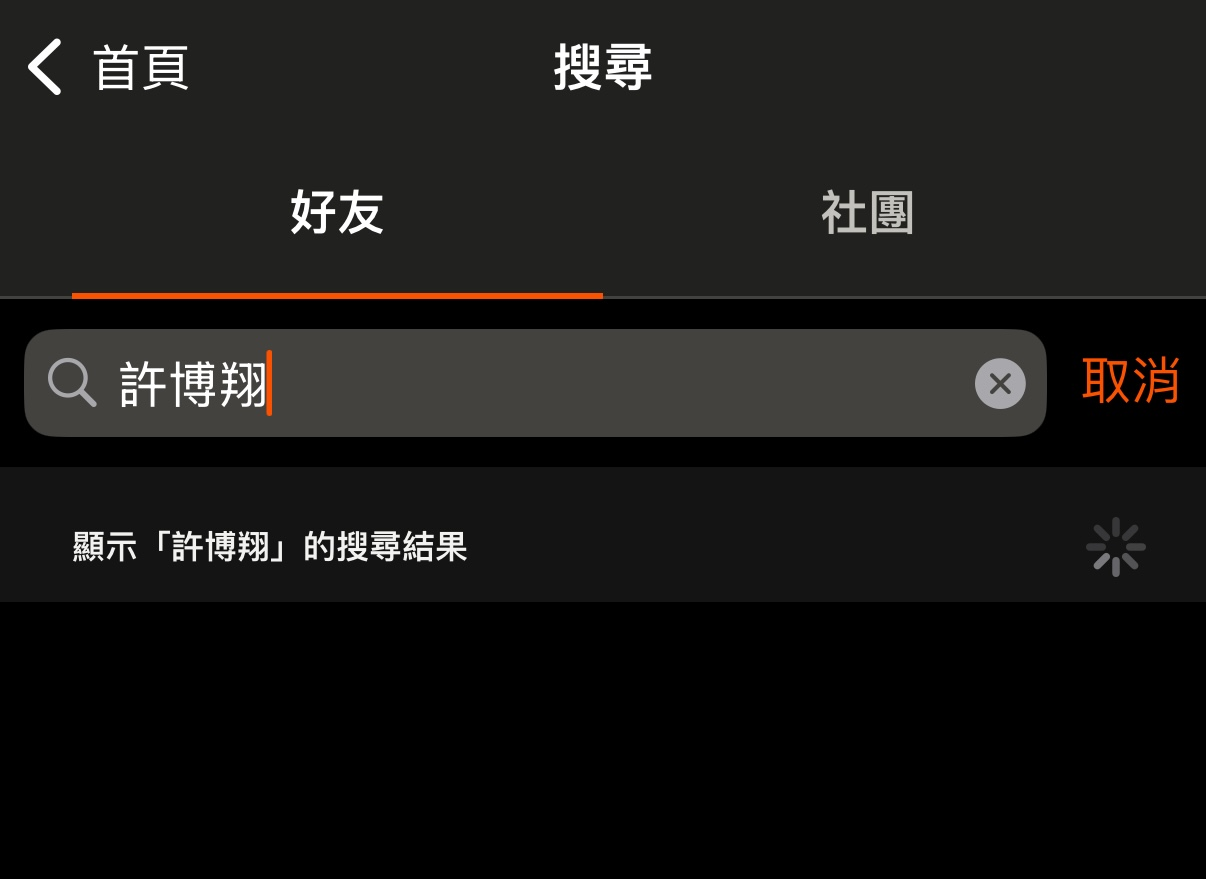
\includegraphics[width=3cm]{search2.png}\\
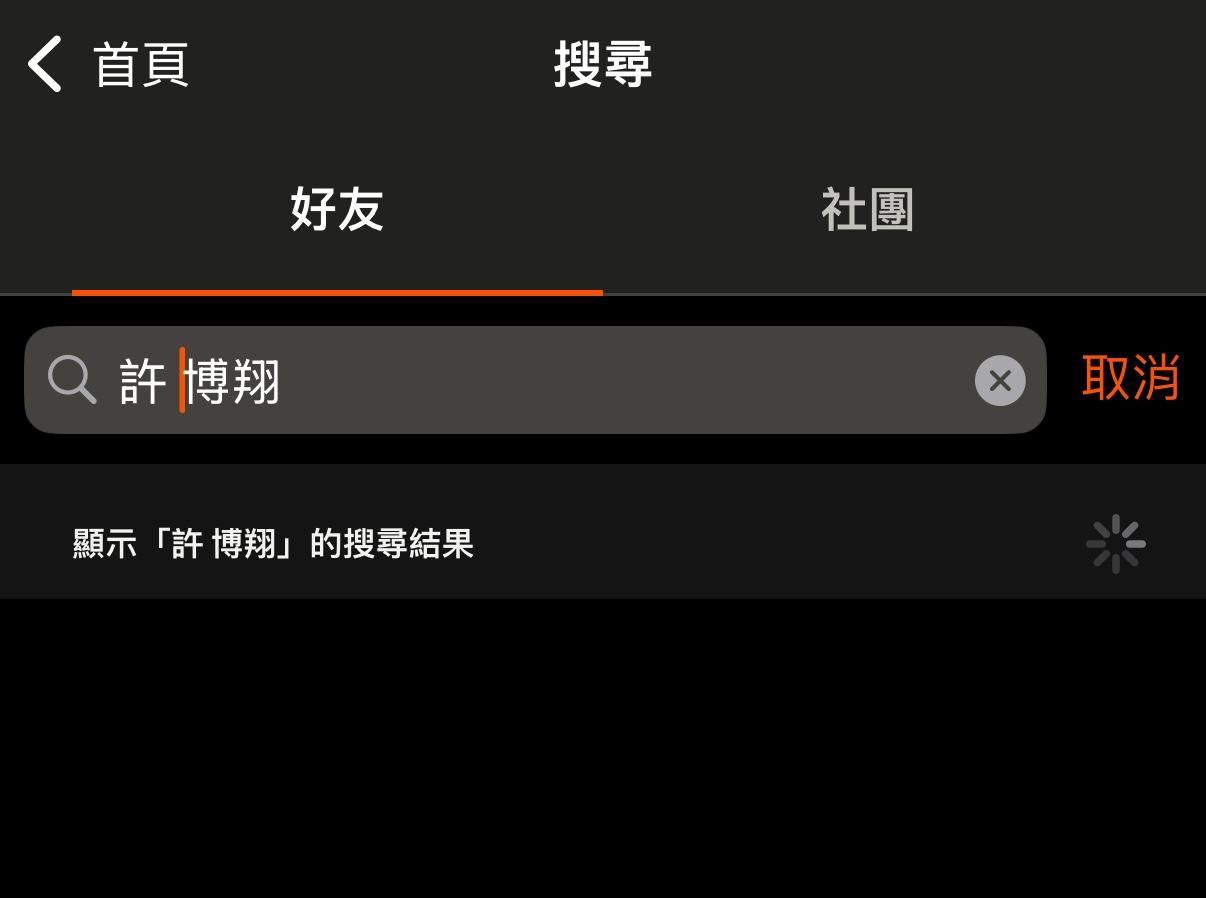
\includegraphics[width=3cm]{search3.png}\\
\end{multicols}
}\only<2>{
\begin{multicols}{2}
\item 加社團\\

\includegraphics[width=3cm]{club.png}
\item 傳訊息\\
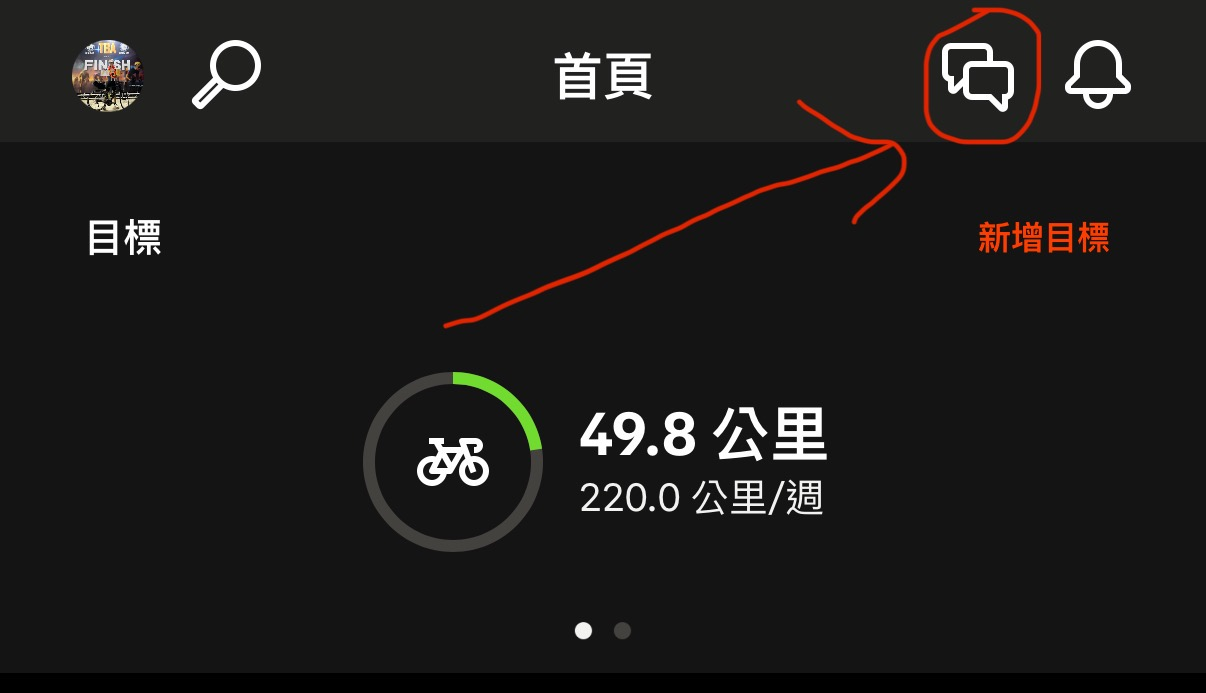
\includegraphics[width=5cm]{message.png}

\includegraphics[width=3cm]{message2.png}
\end{multicols}
}\only<3>{
\begin{multicols}{2}
\item 按讚貼文、留言(貼文的讚無法收回,留言的讚可以收回)
\item 貼文、留言都可以標注人
\item 留言無法編輯,但是可以向右滑刪除/檢舉/回覆
\item 自己貼文底下的留言以及自己的留言可以刪除
\item 別人的留言可以檢舉/回覆
\newpage

\includegraphics[width=3cm]{post.png}

\includegraphics[width=3cm]{post2.png}
\end{multicols}
}\only<4>{
\item \begin{center}\begin{tabular}{c|c}
Strava & Instagram\\\hline
可以加好友 & 可以加好友\\
可以加社團 & 可以加社團\\
可以傳訊息 & 可以傳訊息\\
可以發文 & 可以發文\\
貼文可以放照片 & 貼文可以放照片\\
可以留言 & 可以留言\\
可以按讚貼文/留言 & 可以按讚貼文/留言\\
可以刪除貼文/留言 & 可以刪除貼文/留言\\
可以放地圖 & 不能放地圖\\
可以刷路段 & 不能刷路段\\
可以計算運動的數據 & 無法計算運動的數據\\
不會被祖 & 可能會被祖
\end{tabular}\end{center}
}
\end{itemize}
\end{frame}

\begin{frame}{團體活動}
\begin{multicols}{2}
\begin{itemize}
\item 忘了紀錄活動或是紀錄有問題怎麼辦?請一起運動的朋友標注你\\

\includegraphics[width=3cm]{rideTogether.png}

\includegraphics[width=3cm]{rideTogether2.png}
\newpage
\item 如果A在某個活動中有$50\%$以上的時間是在B的某個活動的附近,那 Strava 會在A的活動中說與B一起騎乘
\item 是否一起騎乘並不是對稱的(在數學上的說法是並非等價關係)\\
{\tiny 等價關係是指具有自反性、對稱性、遞移性的二元關係}\\
舉例來說,A的某個活動是跟了B的某個$24$小時的活動的最前面$8$的小時(例如B騎一日台九而A騎一日北花),那在A的活動中會寫跟B一起騎乘,但是在B的活動中不會寫跟A一起騎乘
\end{itemize}
\end{multicols}
\end{frame}

\begin{frame}{尋找活動}
\begin{itemize}
\only<1>{
\item 依照名稱尋找(僅限自己的活動)\\
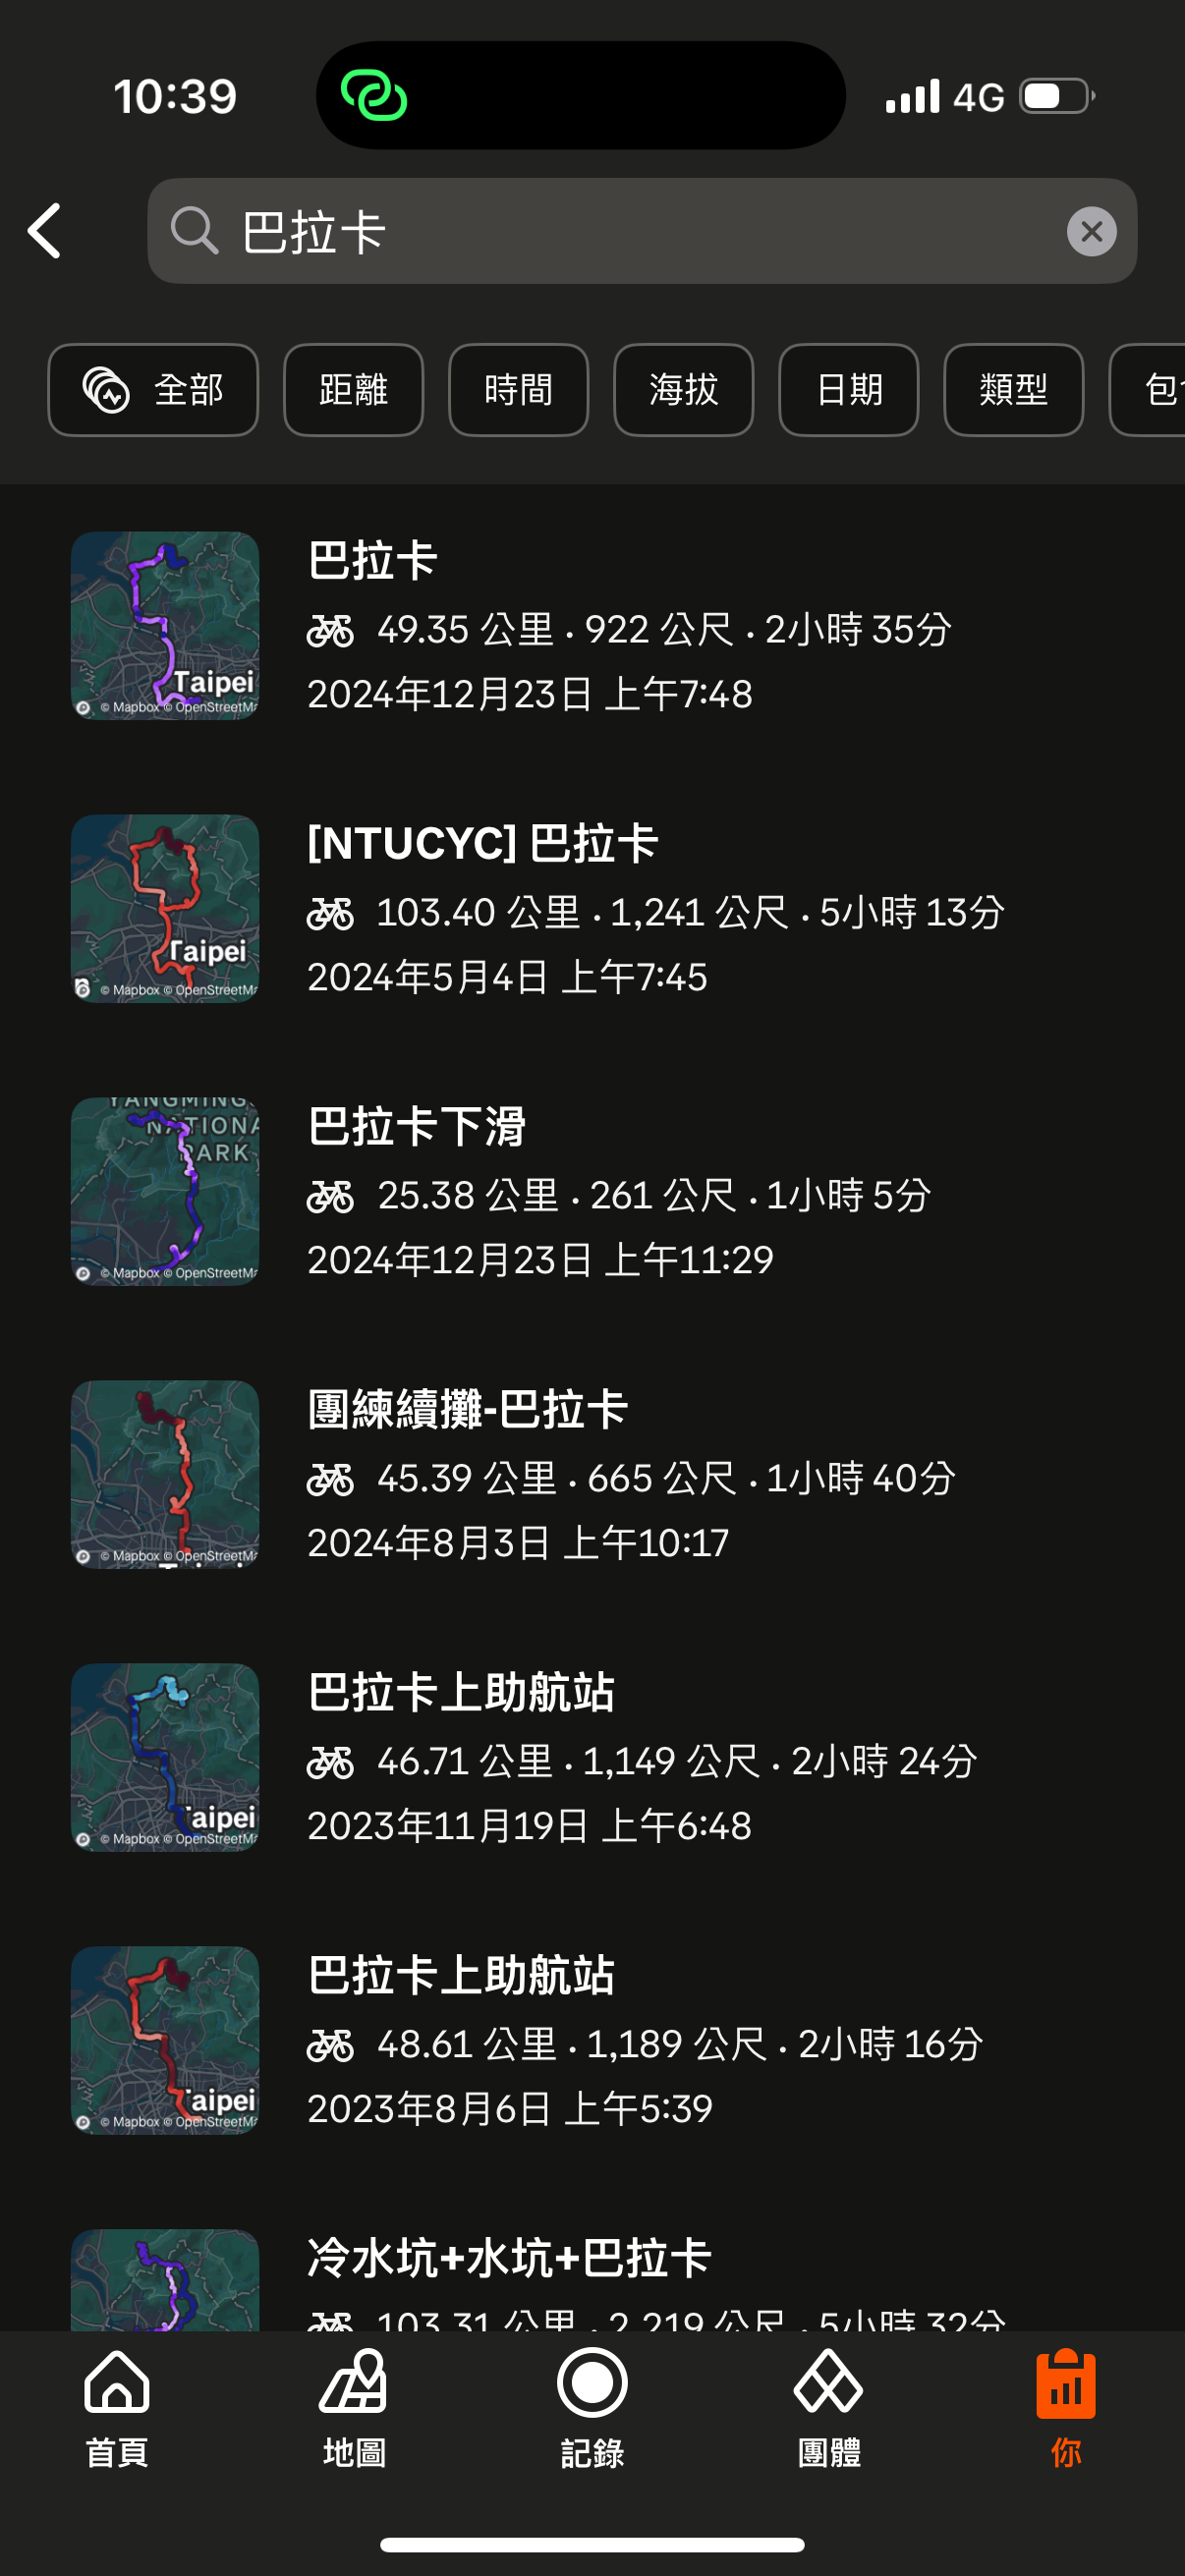
\includegraphics[width=3cm]{getActivityByName.png}
}\only<2>{
\begin{multicols}{2}
\item 依照時間尋找(網頁版)\\
\begin{itemize}
\item 自己的:點右上角頭貼,然後點「My Profile」
\item 別人的:左上角搜尋那個人,搜完之後就看到了
\end{itemize}
點你要找的時間對應的那一條,會顯示所有在那一週的活動
\newpage
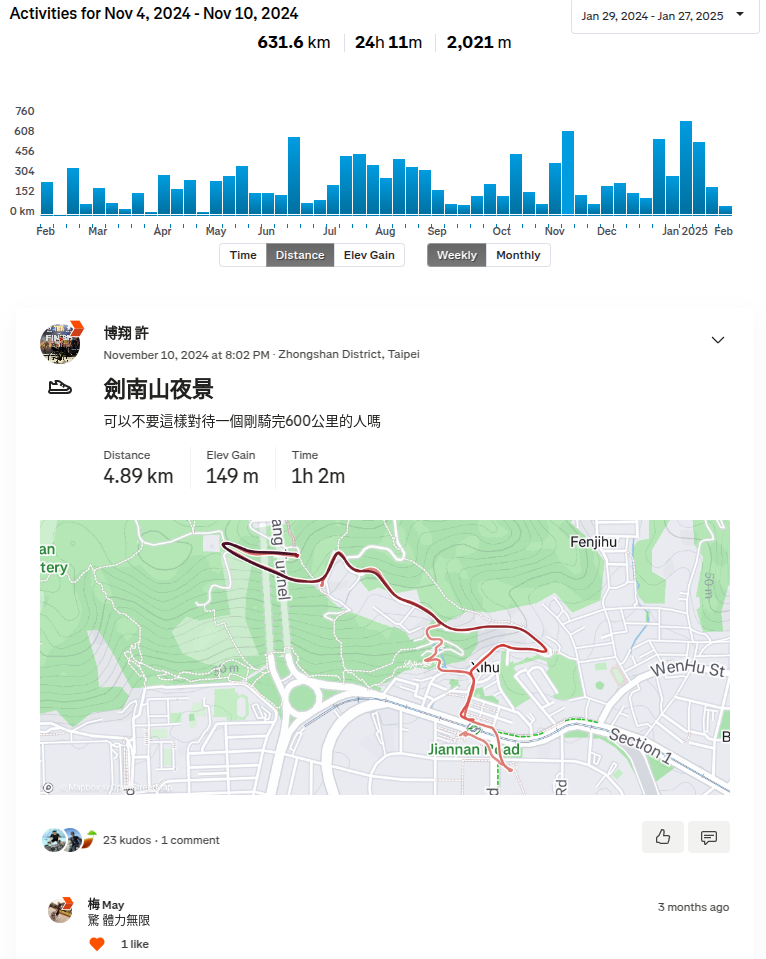
\includegraphics[width=5cm]{getActivityByTime.png}
\end{multicols}
}
\end{itemize}
\end{frame}

\begin{frame}{播放活動}
\begin{itemize}
\item 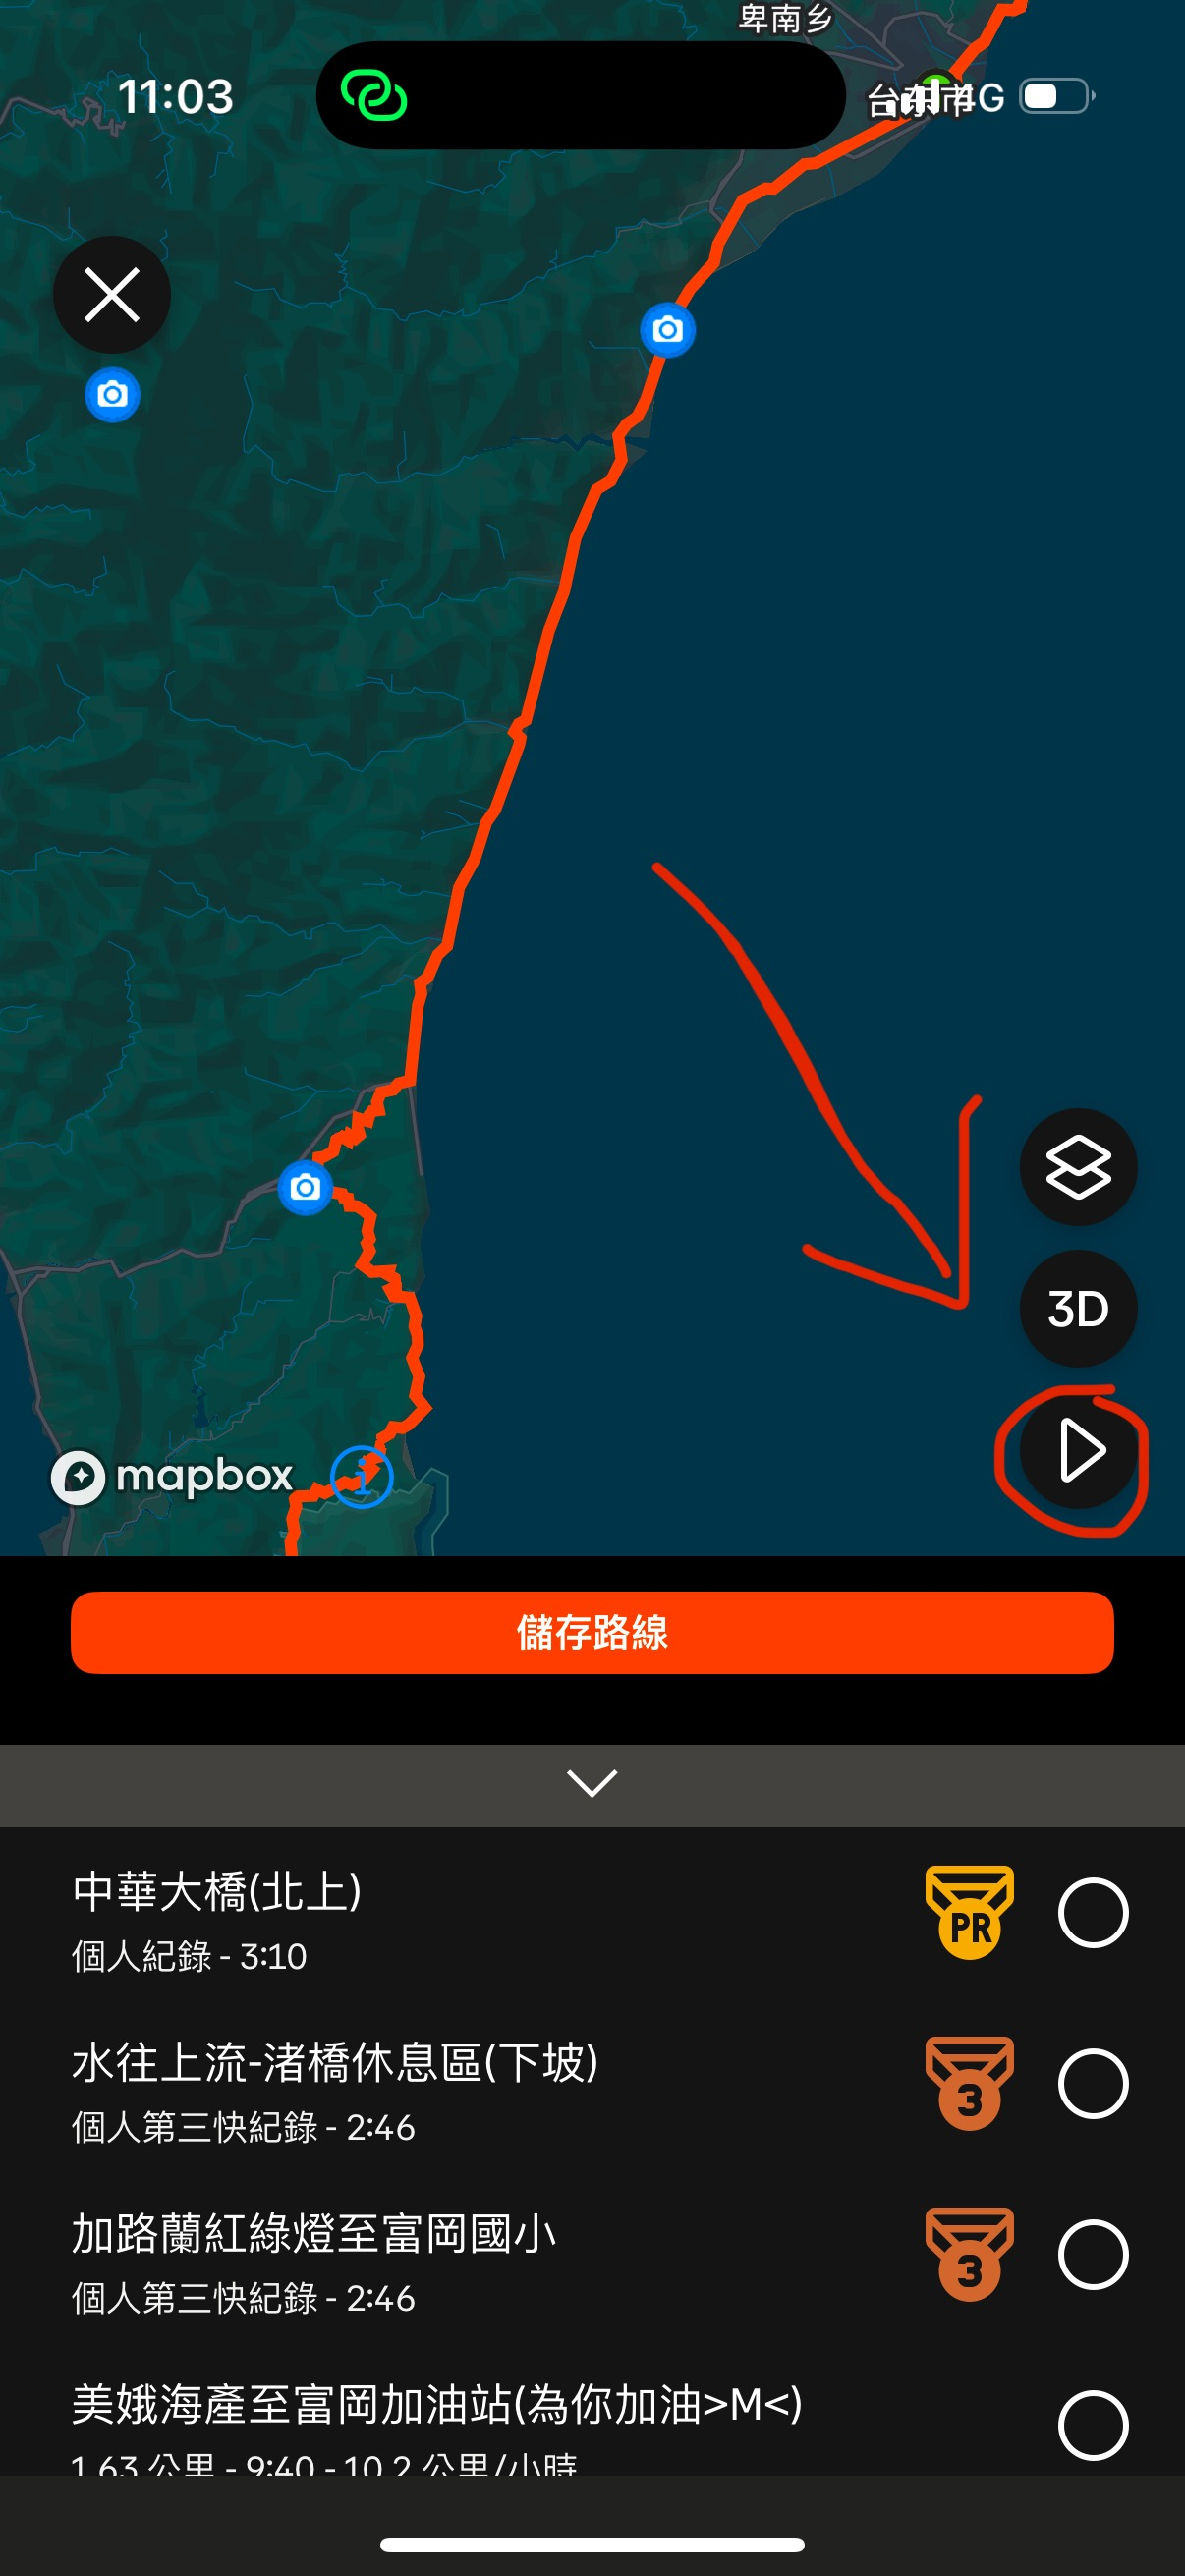
\includegraphics[width=3.2cm]{playActivity.png}
\includegraphics[width=3.2cm]{playActivityWuling.png}
\includegraphics[width=3.2cm]{playActivityTaitung.png}
\includegraphics[width=3.2cm]{playActivityTataka.png}
\end{itemize}
\end{frame}

\section{外掛程式}

\begin{frame}{Statshunter}
\only<1>{
\begin{multicols}{2}
\begin{itemize}
\item 網頁:\url{https://www.statshunters.com}

\includegraphics[width=3cm]{QRcodeStats.png}
\item Heatmap:所有騎過的路線畫出的地圖
\end{itemize}
\newpage
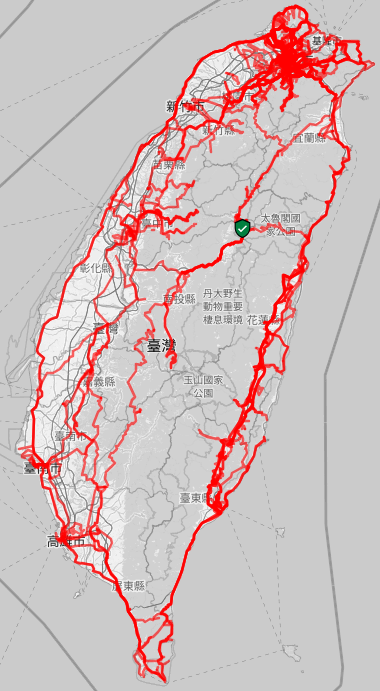
\includegraphics[height=6.5cm]{statsTaiwan.png}
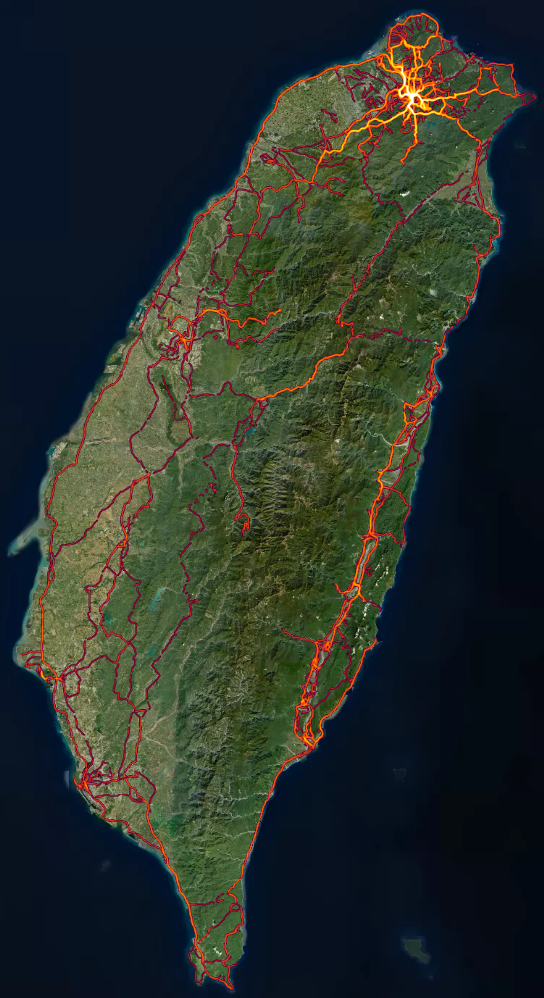
\includegraphics[height=6.5cm]{taiwanHeatmap.png}
\end{multicols}
}\only<2>{
\begin{itemize}
\item Explore tiles:Statshunter 會把整個地球切成$2^{14}\times2^{14}$個(近似)正方形的格子\\
格子的寬度$=$赤道長度$\times\cos($緯度$)\times2^{-14}\approx2.446\times\cos($緯度$)km$\\
\item 在台北一格大約是$2.217km\times2.217km$,而在奧克蘭一格大約是$1.957km\times1.957km$
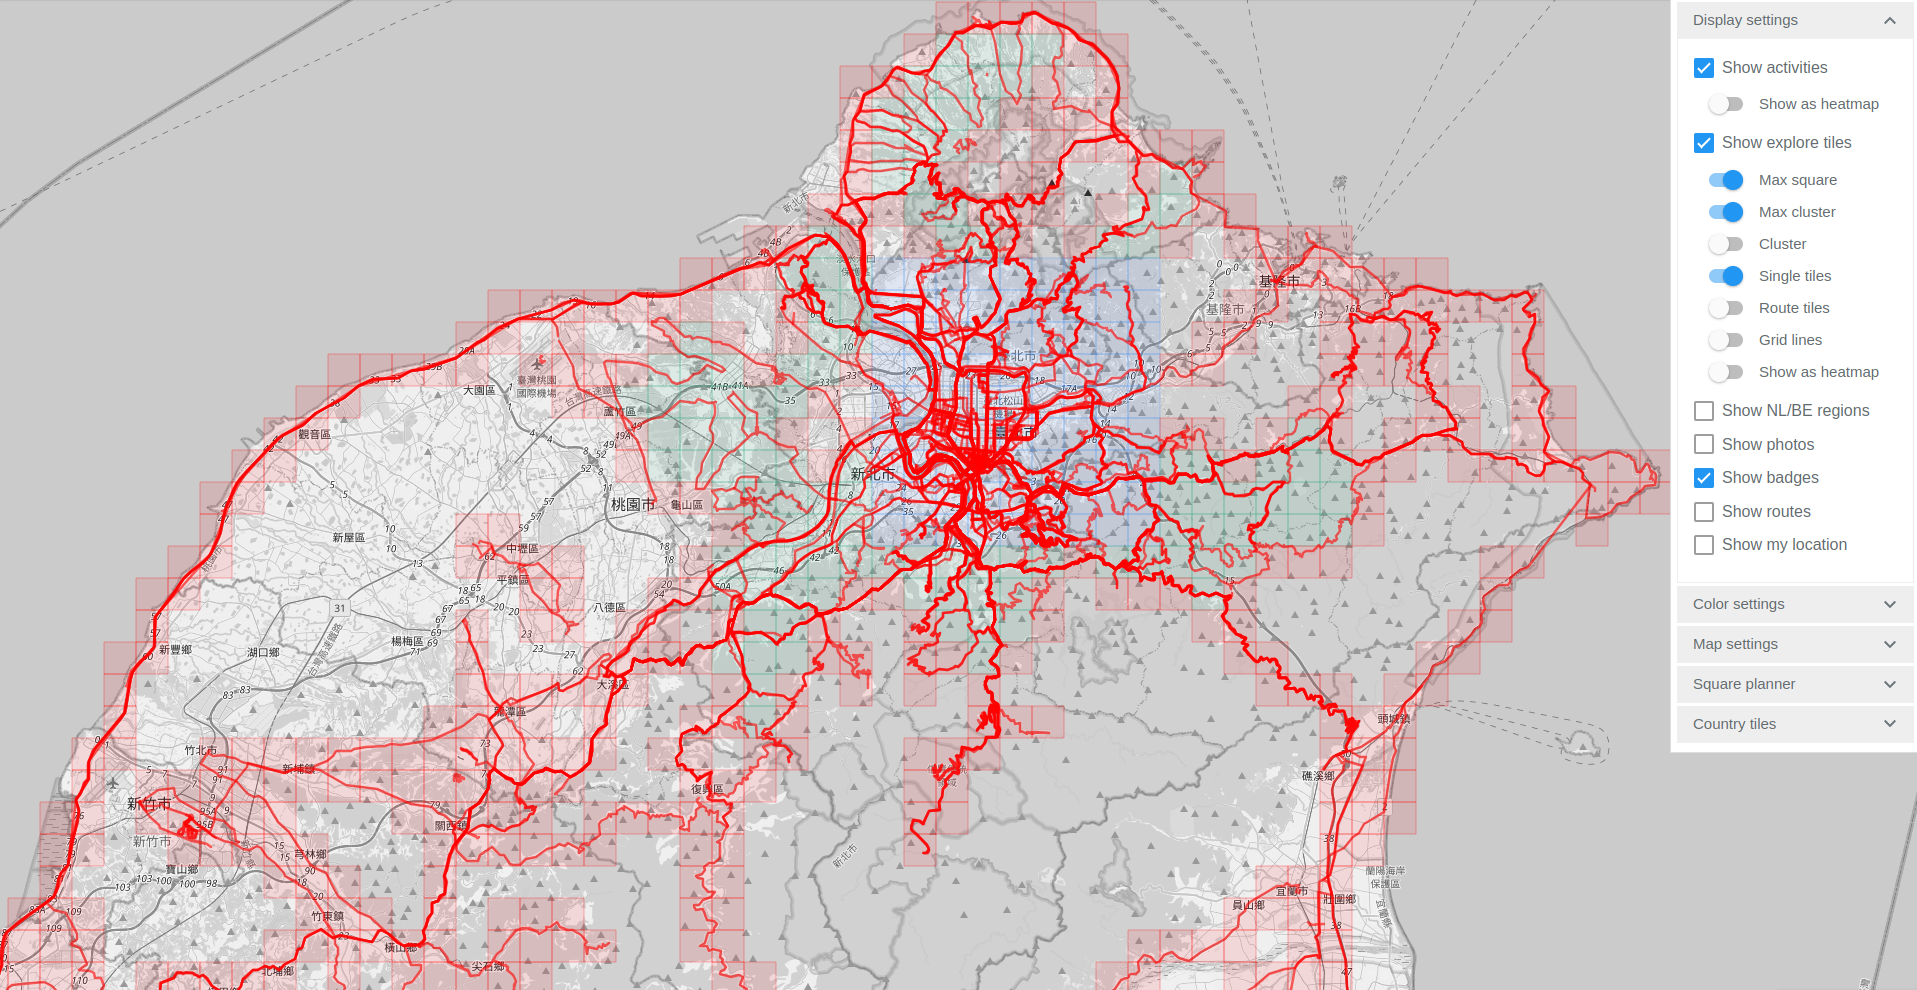
\includegraphics[width=11cm]{statsTaipei.png}
\end{itemize}
}\only<3>{
\begin{multicols}{2}
\begin{itemize}
\item Filter:比如說你可能只想看某段時間內的 heatmap 、統計數據\\
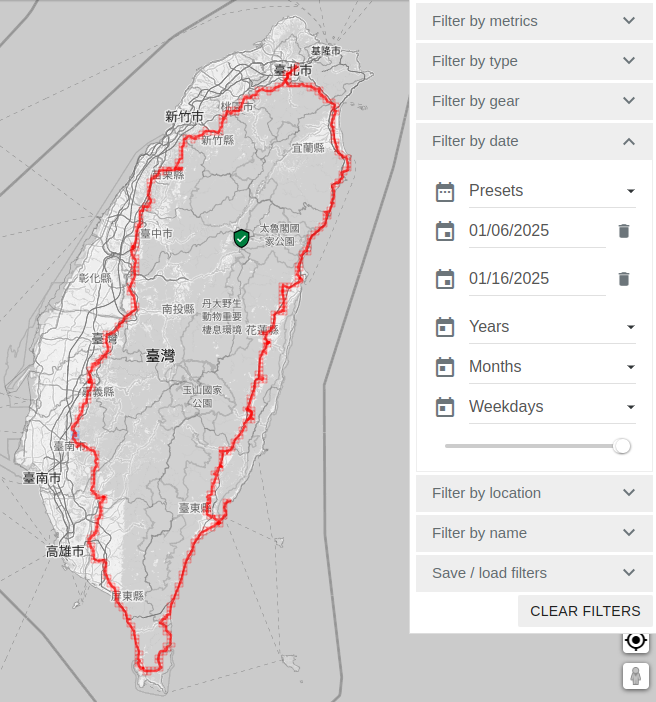
\includegraphics[height=4.5cm]{filterTaiwan.png}
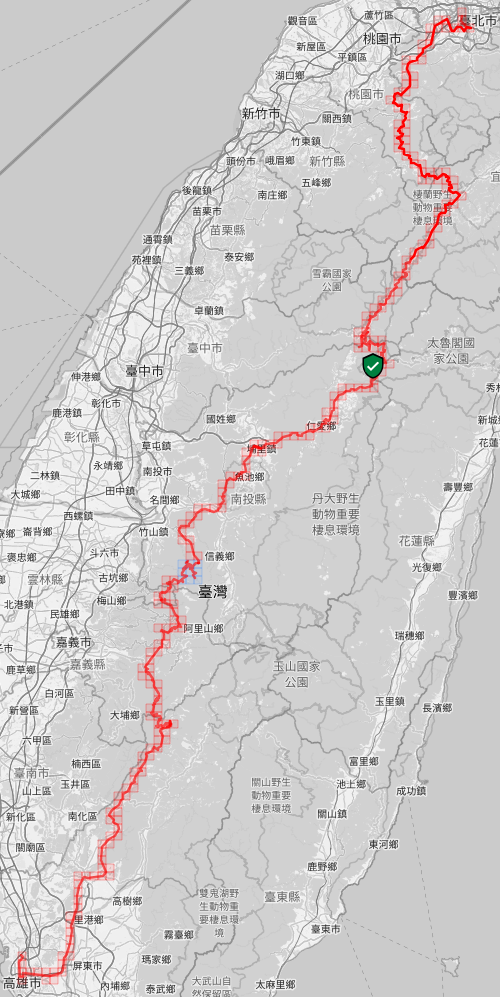
\includegraphics[height=4.5cm]{filterRoof.png}
\end{itemize}
\newpage
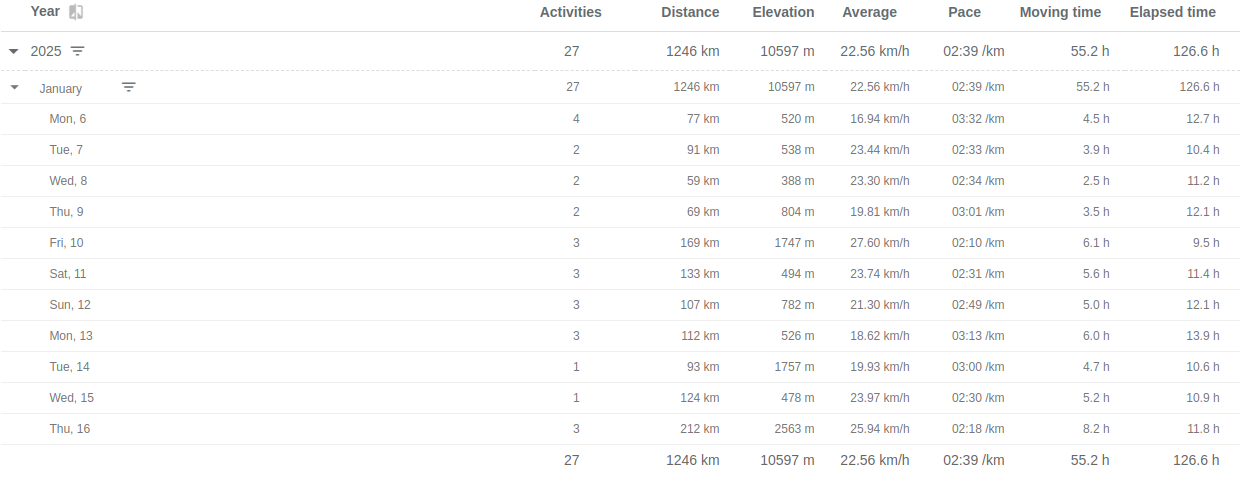
\includegraphics[width=7cm]{filterTaiwanStats.png}
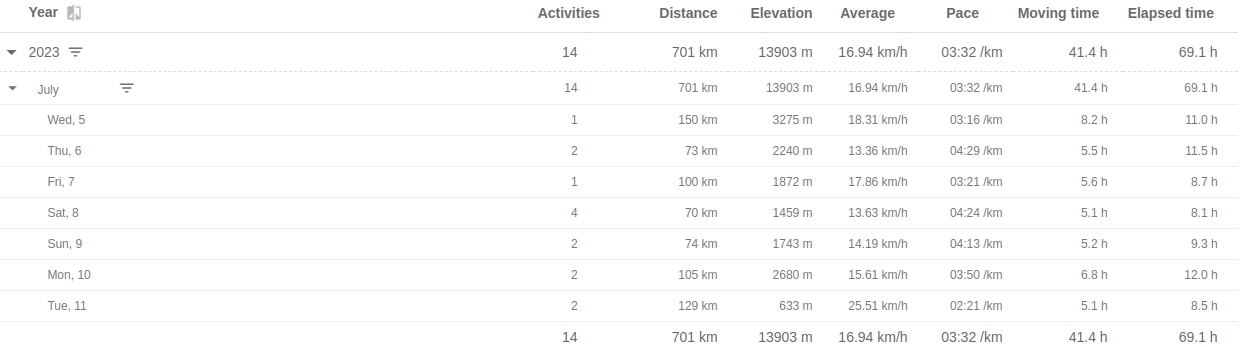
\includegraphics[width=7cm]{filterRoofStats.png}
\end{multicols}
}\only<4>{
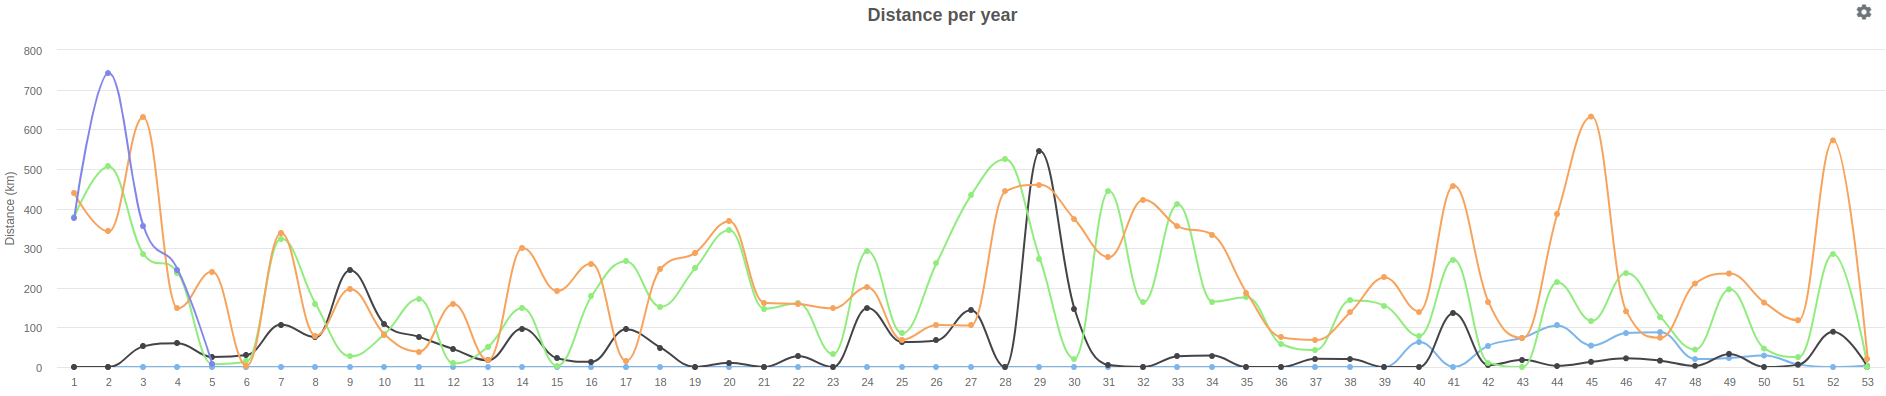
\includegraphics[width=15cm]{statsDistance.png}
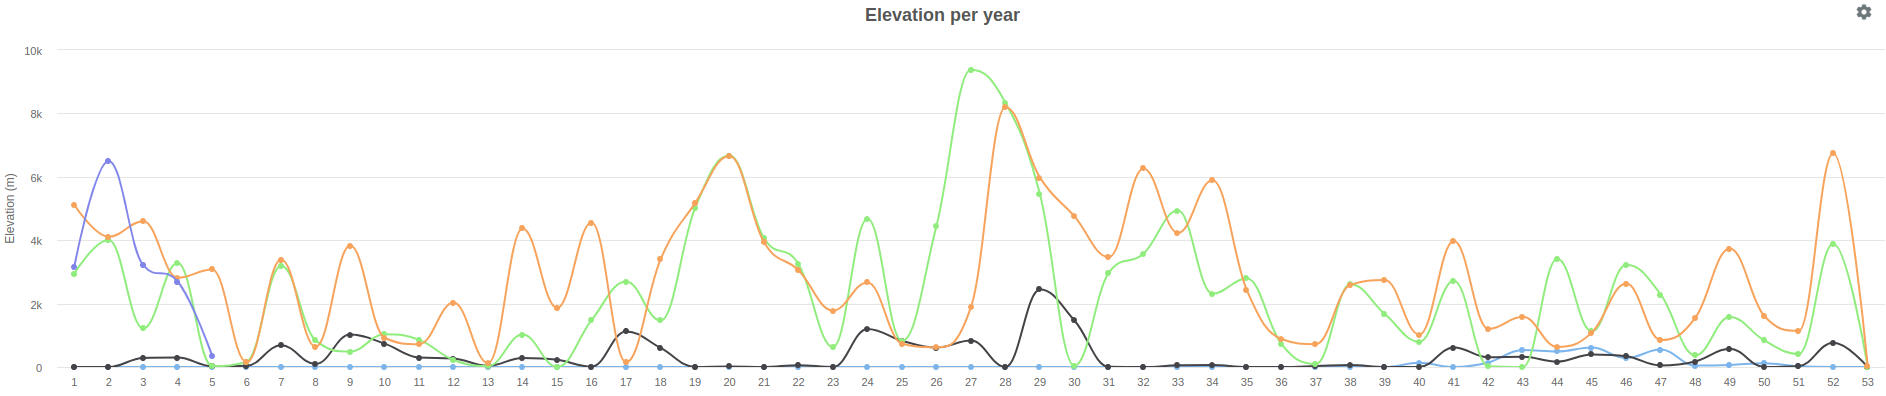
\includegraphics[width=15cm]{statsElevation.png}
}\only<5>{
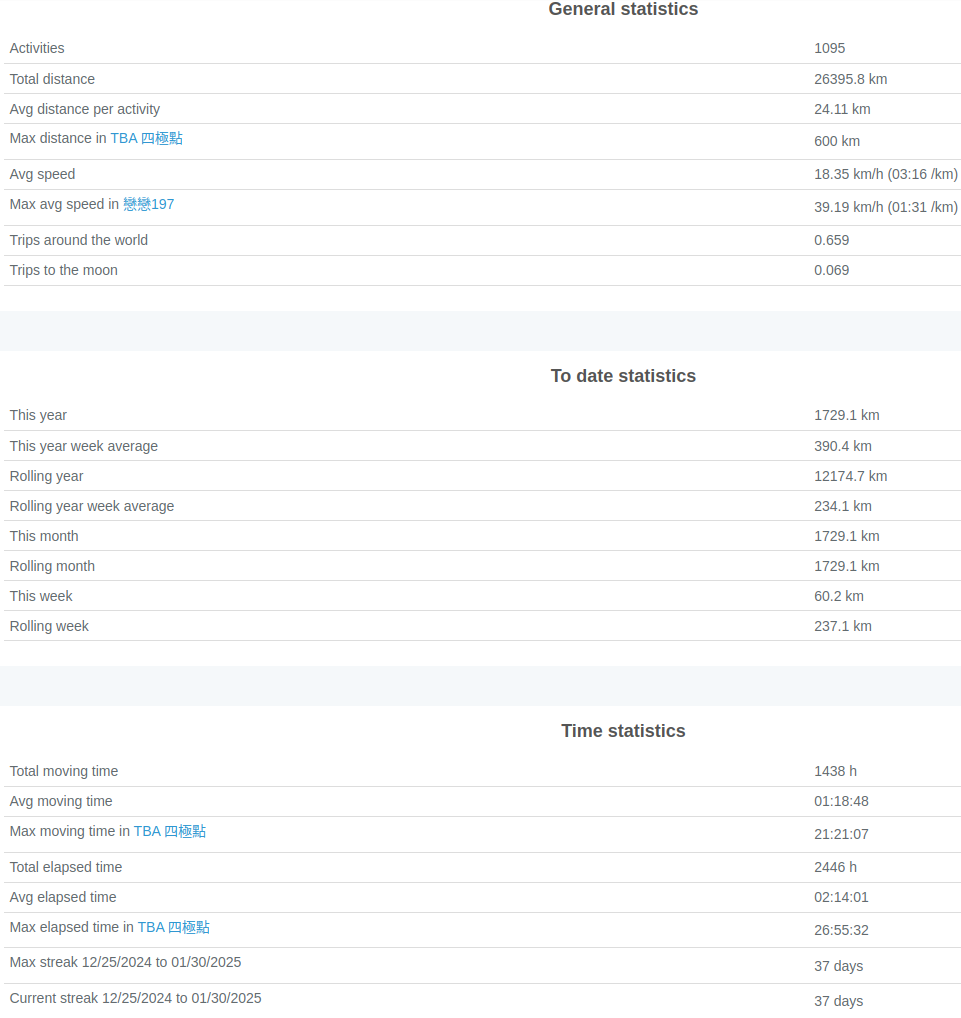
\includegraphics[height=7cm]{statsAll.png}
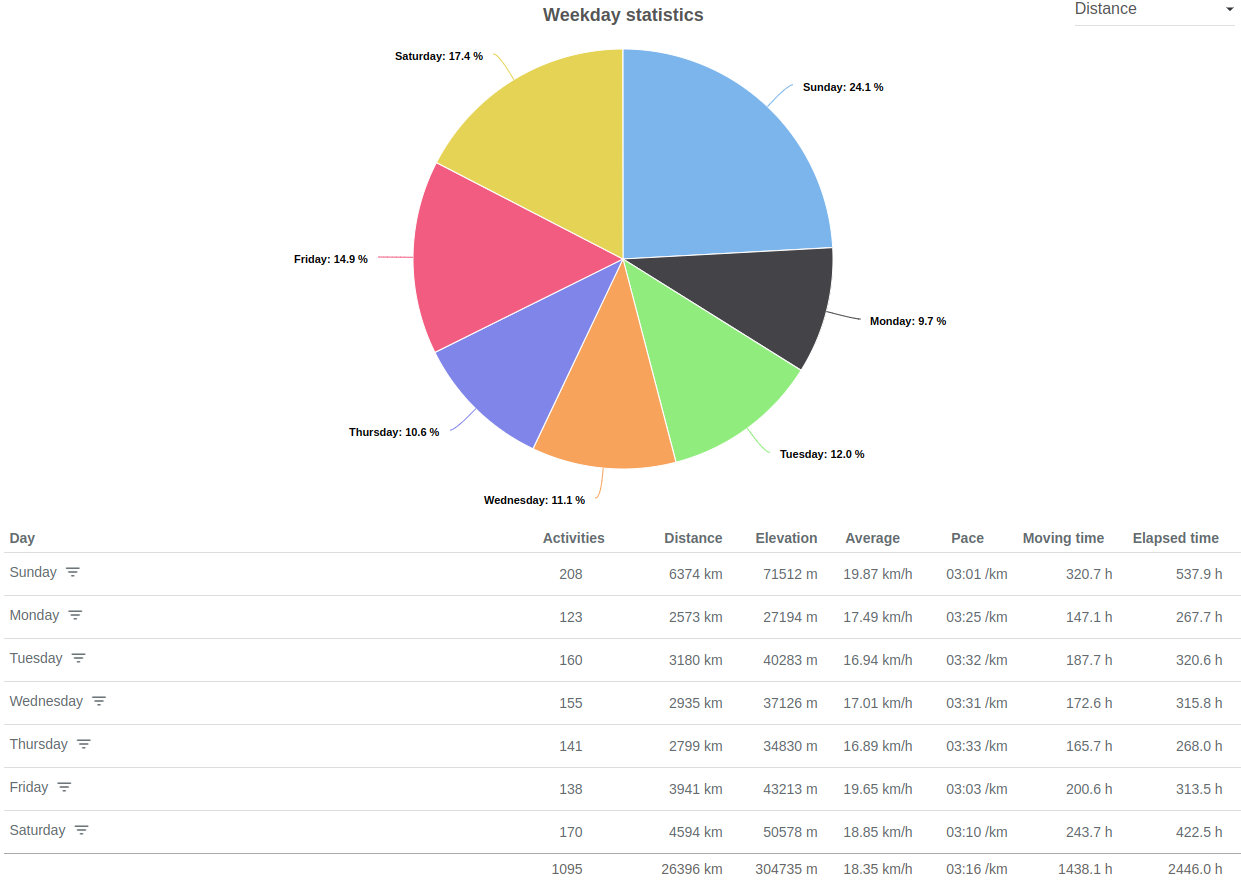
\includegraphics[height=6cm]{statsWeek.png}
}\only<6>{
\includegraphics[width=7.5cm]{statshour.png}
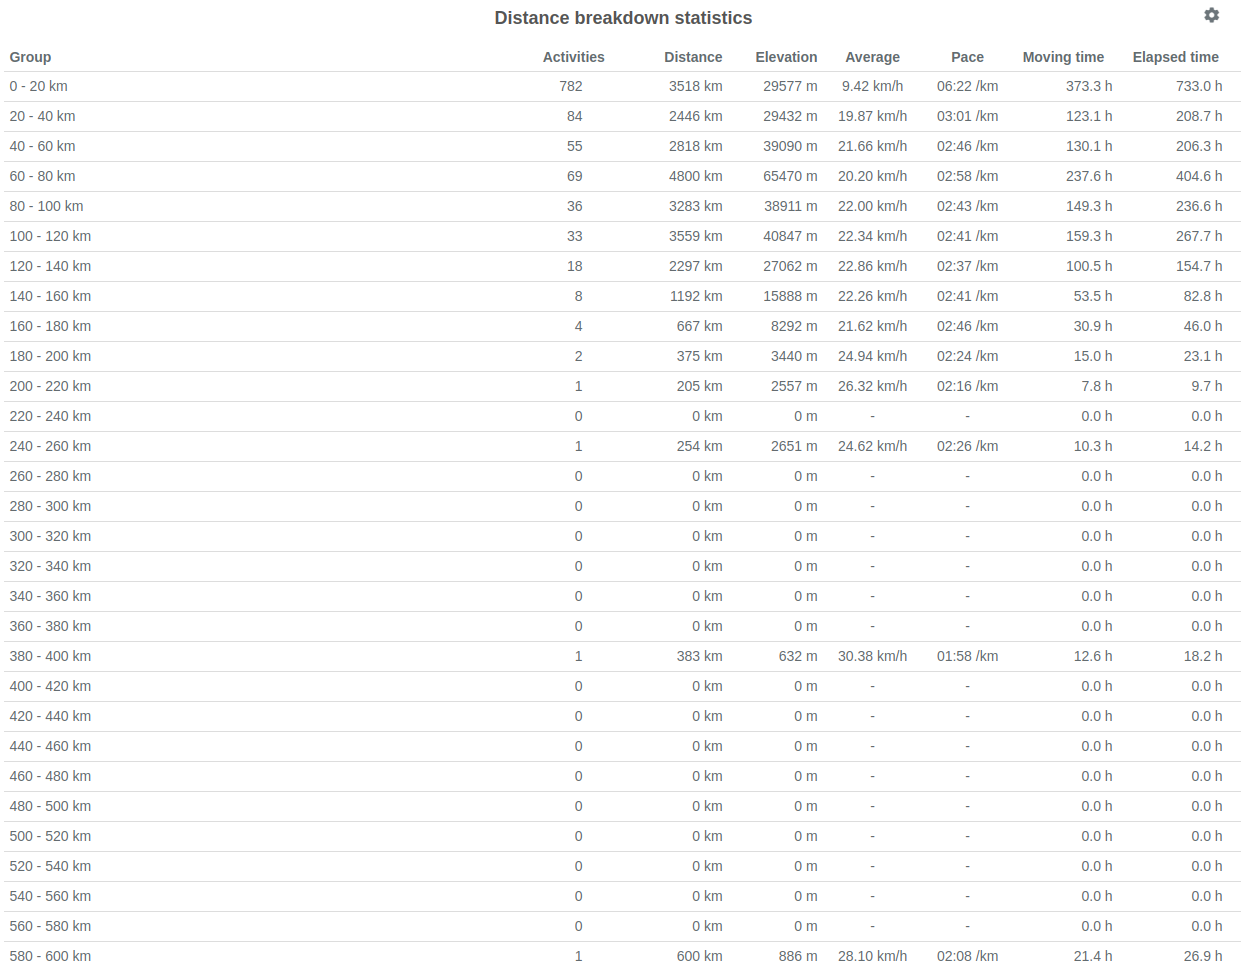
\includegraphics[width=7.5cm]{distanceBreakdown.png}
}
\end{frame}

\begin{frame}{Flyby}
\begin{itemize}
\item 打開方法:設定$\to$隱私控管功能$\to$Flyby$\to$所有人
\item 用上帝視角看在某個特定時間點所有的人分別在哪裡
\item 比對每個人的領先/落後的狀況
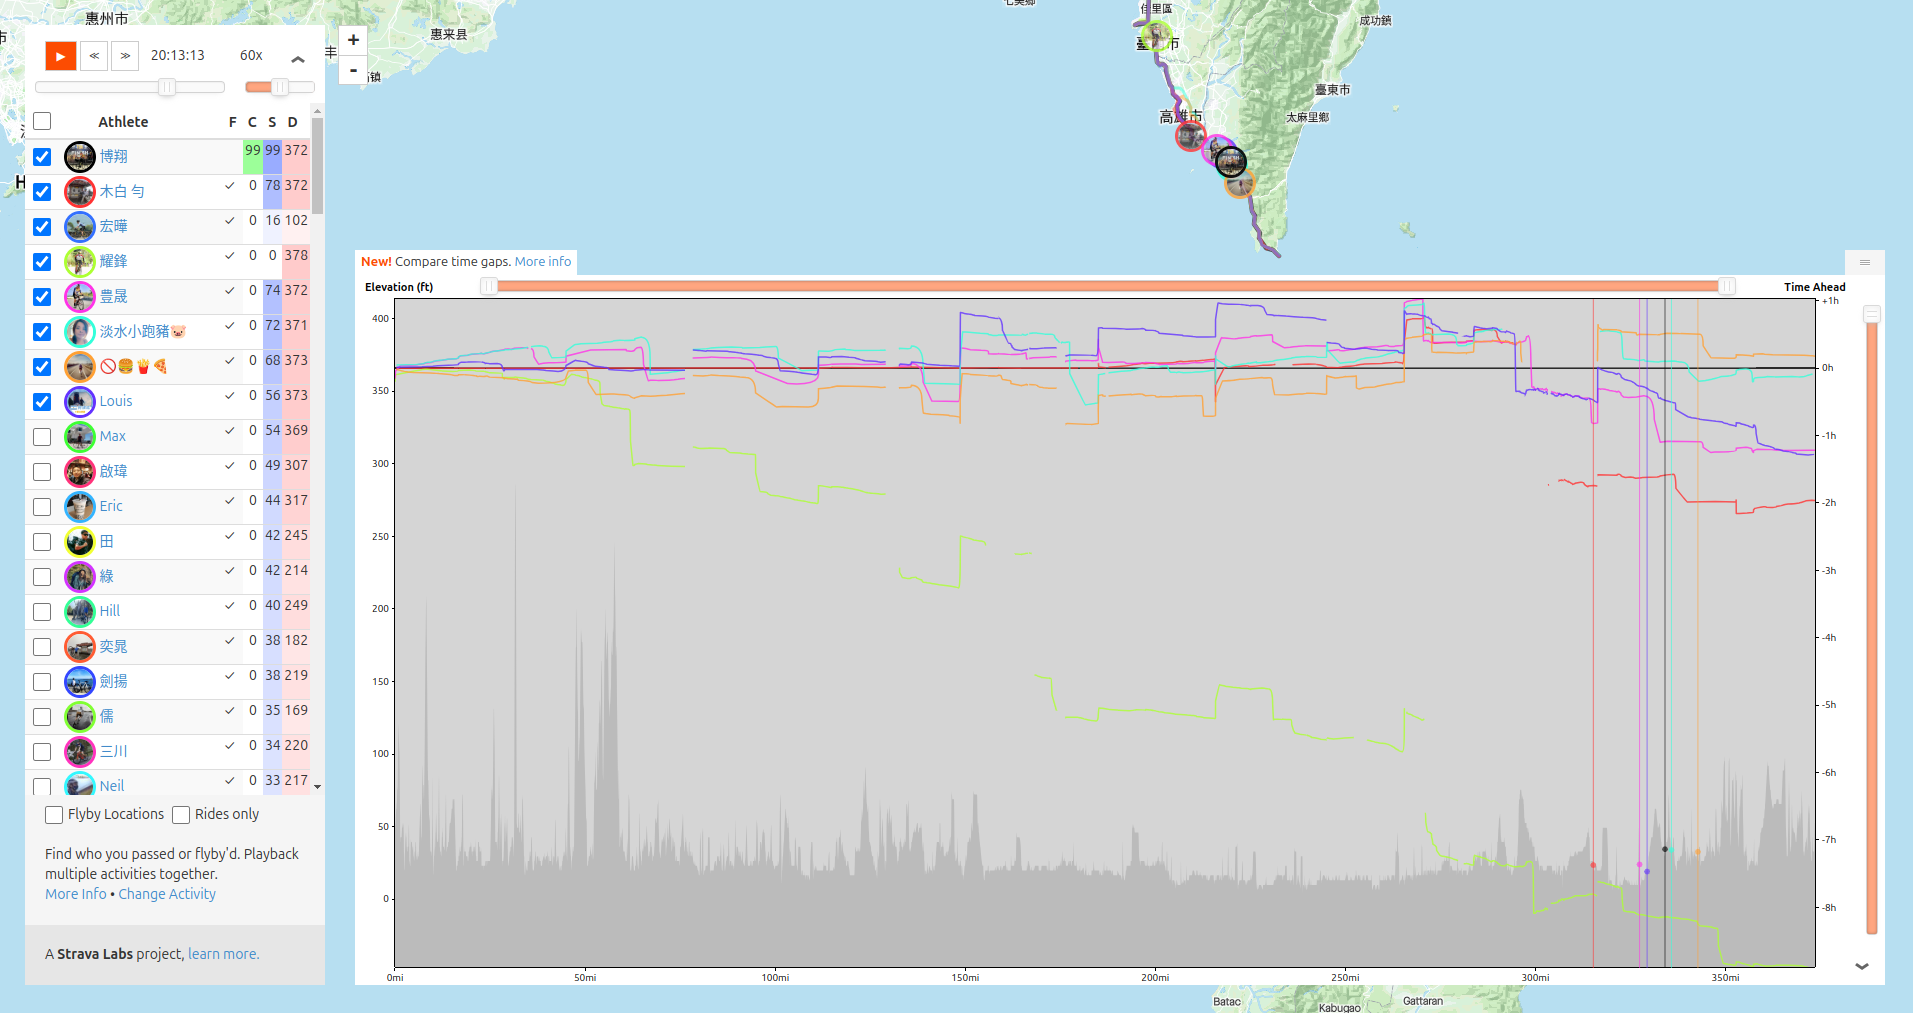
\includegraphics[width=11cm]{flyby.png}
\end{itemize}
\end{frame}

\begin{frame}{Intervals}
\begin{itemize}
\only<2>{
\item 分析訓練強度
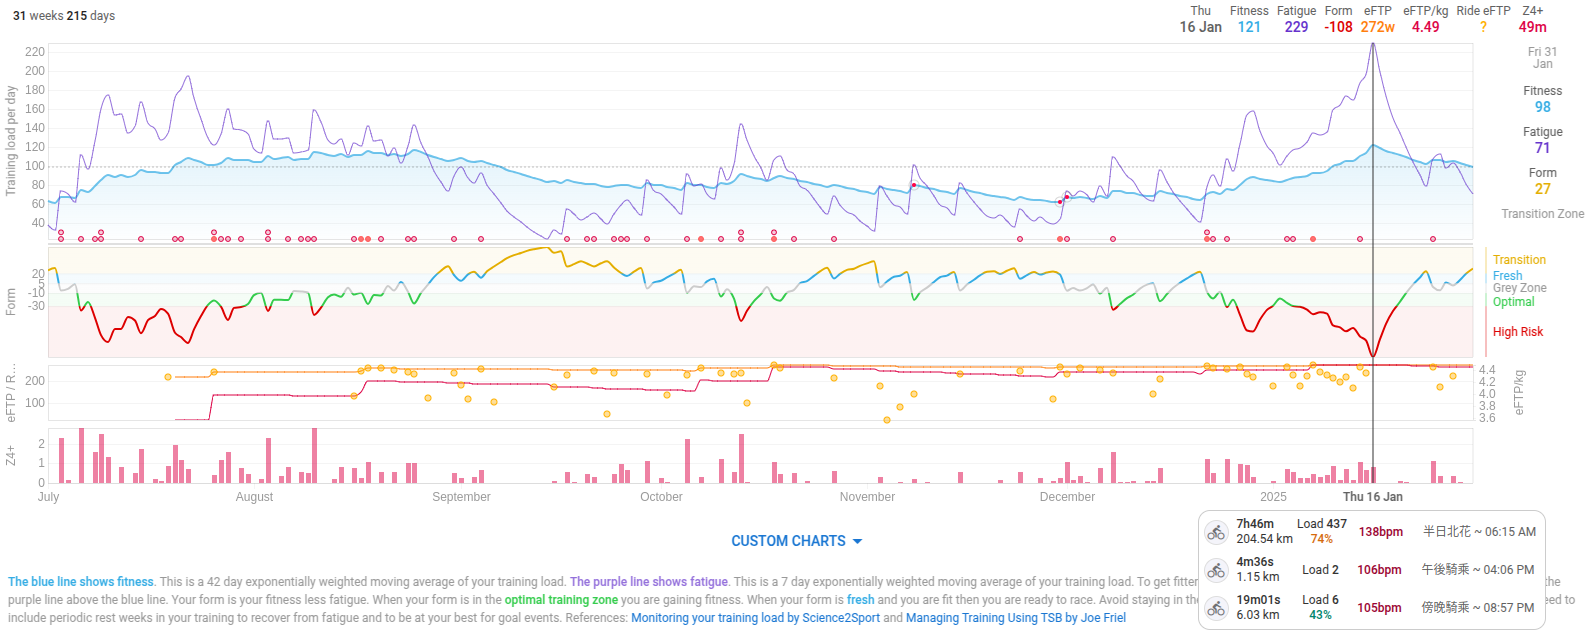
\includegraphics[width=14cm]{intervalsFitness.png}
}\only<1>{
\item 分析功率、心率資料
\item 估計FTP
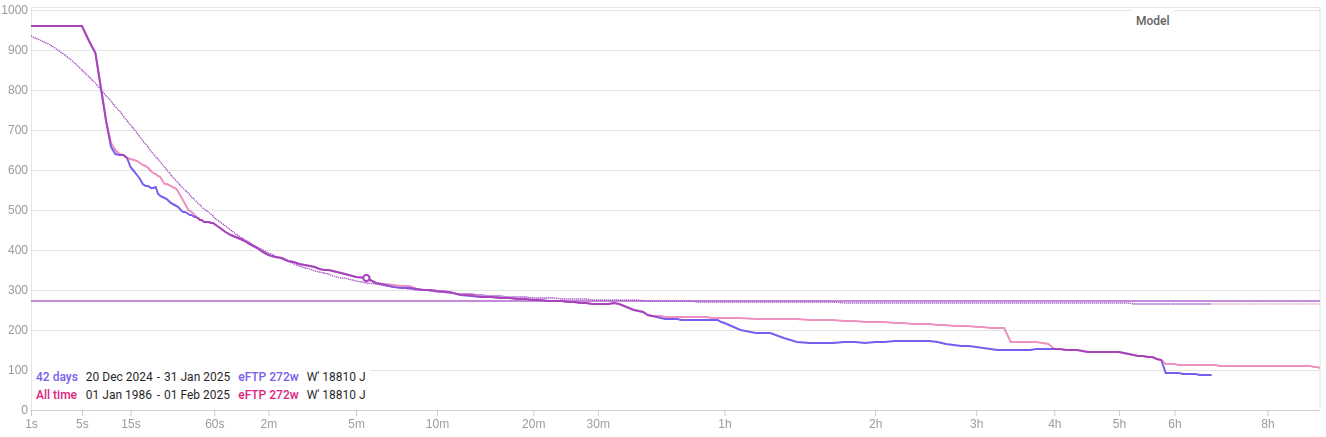
\includegraphics[width=14cm]{intervalsPower.png}
}
\end{itemize}
\end{frame}


\section{路段}

\begin{frame}{情人節要做什麼}
\begin{center}

\includegraphics[height=7cm]{holdmeme.JPG}
\end{center}
\end{frame}

\begin{frame}{路段 (Segment)}
\begin{itemize}
\item 一條大家常常騎的路
\item 通常是爬坡、比賽路線
\item 可以比較大家的成績
\item 常見路段:\href{https://brianhsu7476.github.io/segmentsExplorer/}{Segments Explorer}
\item \includegraphics[height=5cm]{maokongSegment.png}
\includegraphics[height=5cm]{coffeeSegment.png}
\includegraphics[height=5cm]{balakaSegment.png}
\includegraphics[height=5cm]{wulingSegment.png}
\includegraphics[height=4cm]{segmentsExplorer.png}
\end{itemize}
\end{frame}

\begin{frame}{名詞}
\begin{itemize}
\item PR (Personal Record) / PB (Personal Best) :個人(最佳)紀錄
\item 皇冠:在一個路段拿到總排第一名 / 女子第一名,拿到皇冠的稱為登山王 (KOM, King of Mountain) / 登山女王 (QOM, Queen of Mountain)
\item 獎盃:在一個路段拿到總排前十名 / 女子前十名
\item Local Legend: 九十天內在一個路段騎過最多次的人
\item \includegraphics[height=5cm]{KOM.png}
\includegraphics[height=5cm]{KOM2.png}
\includegraphics[height=5cm]{trophy.png}
\includegraphics[height=5cm]{trophy2.png}
\includegraphics[height=5cm]{localLegend.png}
\includegraphics[height=5cm]{localLegend2.png}
\end{itemize}
\end{frame}

\begin{frame}{名詞}
\begin{itemize}
\item \begin{center}\includegraphics[height=7cm]{KOMmeme.jpg}\end{center}
\end{itemize}
\end{frame}

\begin{frame}{排名}
\begin{multicols}{2}
\begin{itemize}
\item 年齡:依年齡分組排名(比如我在20至24歲組)
\item 體重:依體重分組排名(比如我在55至64公斤組)
\item 今年:當年度的排名
\item 今天:當天的排名,如果不是太熱門的路段,通常可以在團騎拿來看各自的速度
\item	正在追蹤:你跟你正在追蹤的人之間的排名,比如如果追蹤新店奧特曼,那可能在大部分的路段名次都會往後一名
\item 社團:可以看自己的社內排名
\newpage
\item \includegraphics[height=7cm]{rank.png}
\includegraphics[height=7cm]{rank2.png}
\end{itemize}
\end{multicols}
\end{frame}

\begin{frame}{計時原理}
\begin{multicols}{2}
\begin{itemize}
\item 路段時間$=$通過終點的時間$-$通過起點的時間
\item 通過起/終點判定
\begin{itemize}
\item 活動:由一堆點(通常一秒一個)組成的一條折線
\item 通過起/終點:這些點與起/終點距離的 local minimum ,也就是在一個區間之內與起/終點距離最近的點
\end{itemize}
\item 計時狀態:通過起點之後,依序抵達路段中的各個點,並且未偏離路段太遠
\item 計時流程
\begin{itemize}
\item 通過起點
\item 計時狀態
\item 通過終點
\end{itemize}
\newpage
\pause
\item 你以為的路段
\includegraphics[width=5.5cm]{wulingMap.png}
\item 實際上的路段
\includegraphics[width=5.5cm]{maokong3pMap.png}
\end{itemize}
\end{multicols}
\end{frame}

\newcommand{\yes}[1]{\alt<2>{\textcolor{red}{#1}}{\textcolor{black}{#1}}}
\newcommand{\maybe}[1]{\alt<2>{\textcolor{orange}{#1}}{\textcolor{black}{#1}}}

\begin{frame}[fragile]{如何避免計時失敗}
\begin{itemize}
\item 計時失敗: Strava 上的路段時間明顯跟騎的時間不一樣
\item 下列哪些情況容易造成計時失敗?
\begin{enumerate}[A]
\item \yes{在起點休息了一會之後直接上山(例如在萊爾富三芝天涯店休息,休完之後直接計時巴拉卡)}
\item \yes{計時完直接停在終點等待其他隊友(例如爬完助航站直接停在旁邊拍大屯山風景)}
\item \yes{計時到一半折返找隊友}
\item 計時途中停在路邊休息
\item \yes{計時途中岔出去其他地方再回來(例如騎冷水坑途中跑去平菁街看櫻花)}
\item \yes{騎不同條路(例如要計時貓空指南線但騎草湳那條路)}
\item \href{https://www.instagram.com/reel/C5tCGSeyQNI/?utm_source=ig_web_button_share_sheet}{邊計時邊跳舞}
\item \maybe{闖紅燈}
\item \yes{過山洞}
\item \maybe{計時中遇到狗}
\item 計時中搭車
\item \yes{計時中按到暫停}
\end{enumerate}
\end{itemize}
\end{frame}

\begin{frame}{如何避免計時失敗}
\begin{itemize}
\item \sout{在起點休息了一會之後直接上山}\\
出發前先離開起點夠遠的一段距離,再重新進入起點重新開始計時
\item \sout{計時完直接停在終點等待其他隊友}\\
抵達終點之後先離開終點夠遠的一段距離,以確保計時結束
\item \sout{計時到一半折返找隊友}\\
折返時停錶,回到折返點再按錶繼續
\item \sout{計時途中岔出去其他地方再回來}\\
岔出去時停錶,回到出去的點再按錶繼續
\item \sout{騎不同條路}\\
基本上沒救
\item \sout{過山洞}\\
基本上沒救,所以創路段會盡量避免經過過長的山洞
\item \sout{計時中按到暫停}\\
回到按暫停的點按錶繼續計時
\end{itemize}
\end{frame}

\begin{frame}{計時失敗補救}
\begin{itemize}
\item 編輯/裁切活動,重新上傳
\item 把起/終點附近多餘的點拿掉,以讓 Strava 不會把停在那裡休息的點也算進去
\item 把偏離計時路段的點拿掉,以讓 Strava 不會以為你沒在計時
\end{itemize}
\end{frame}

\begin{frame}{有人作弊怎麼辦}
\begin{itemize}
\begin{multicols}{2}
\only<1>{
\item 檢舉他!檢舉完之後他就會從排行榜上消失了。
\item 素材:\href{https://www.strava.com/athletes/117279779}{曹翊}
\item \includegraphics[width=7cm]{flag0.png}
}\only<2>{
\item 點選三個點(Actions)然後選擇 Flag :\\\includegraphics[width=7cm]{flag1.png}
\item 點選檢舉類型並輸入原因:\\\includegraphics[width=7cm]{flag2.png}
}
\end{multicols}
\only<2>{
\item \includegraphics[width=14cm]{flag3.png}
}
\end{itemize}
\end{frame}

\begin{frame}{不要亂檢舉}
\begin{multicols}{2}
\includegraphics[width=7cm]{flag5.png}
\newpage
\includegraphics[width=7cm]{flag4.png}
\end{multicols}
\end{frame}

\section{訂閱功能}

\begin{frame}{活動數據分析}
\only<1-10>{
\begin{itemize}
\item 照著功率/心率/速度/坡度/溫度等數據的高低畫出的地圖\pause
\item 功率區間/心率區間/區段配速\\\pause
\includegraphics[height=5cm]{subscribe1.png}\pause
\includegraphics[height=5cm]{subscribe2.png}\pause
\includegraphics[height=5cm]{subscribe3.png}\pause
\includegraphics[height=5cm]{subscribe4.png}\pause
\includegraphics[height=5cm]{subscribe5.png}\pause
\includegraphics[height=5cm]{subscribe6.png}\pause
\item 其實只要有 GPX 檔,這些都可以自己做\pause
\item Intervals 也有類似的功能
\end{itemize}
}\only<11>{
\includegraphics[height=6cm]{colorMap.png}
\includegraphics[height=6cm]{subscribeStats.png}
}
\end{frame}

\begin{frame}{路段排行榜}
\begin{multicols}{2}
\begin{itemize}
\item 沒訂閱只能看到男女排行榜上的前十名\pause
\item 訂閱可以看到 依年齡、體重、今天、今年、正在追蹤、社團 的排行榜,而且網頁版可以看到完整而非只有前10名的排行榜\pause
\item \href{http://ws1.csie.ntu.edu.tw:9480}{Who Is the 80 King?}:稍微完整一些的排行榜,收集了有標星號的路段,有追蹤或是有在台大單車社 Strava 社團裡的人都會出現在排行榜上\\
\includegraphics[height=3cm]{80KingQRCode.png}
\newpage
\includegraphics[height=7cm]{80King.png}
\end{itemize}
\end{multicols}
\end{frame}

\begin{frame}{路段創建(網頁版)}
\begin{itemize}
\item 當你發現某個很有趣的路段(例如118神掌,或是一條沒人探索過的山路)想與其他人競速,訂閱可以創建路段\pause
\item 創建路段的起終點不要設在太極限的位置以防計時失敗\pause
\item 盡量避免路段經過太長的山洞\\\pause
\includegraphics[height=5cm]{segmentCreate1.png}\pause
\includegraphics[height=5cm]{segmentCreate2.png}
\end{itemize}
\end{frame}

\begin{frame}{路線繪製}
\begin{itemize}
\item 訂閱可以繪製路線\pause
\item Strava 的路線會照 global heatmap 去畫,所以畫出來的路線會是車友常騎的路線\pause
\item Strava 會告訴你一條路線的路況大致上如何\\\pause
\includegraphics[height=6cm]{routeCreate.png}
\end{itemize}
\end{frame}

\section{活動編輯}

\begin{frame}{活動編輯}
\begin{itemize}
\item 上火車之後忘了停錶\pause
\item 想獨立出畫圖的那段活動(比如把騎去泰北高中以及從泰北高中騎回宿舍的部份從神掌的活動中獨立出來)\pause
\item 想獨立出比賽的那段活動(比如開賽前$10$秒就會先按錶,但是那$10$秒影響了 Strava 上看到的成績)\pause
\item 計時失敗\pause
\item 想把畫圖騎錯路的地方刪掉\pause
\item 活動分成了兩段紀錄,想合併成一個活動(比如騎到助航站之後很興奮就先上傳活動了,回去之後想把去程與回程的合併在一起)
\end{itemize}
\end{frame}

\begin{frame}{Strava 內建功能(網頁版)}
\begin{multicols}{2}
\begin{itemize}
\only<1>{
\item 點三個點$\to$Crop/Split
\item Crop:裁切
\item Split:分割
\newpage
\includegraphics[height=6cm]{cropSplit.png}
}\only<2->{
\pause
\item 裁切:去頭去尾\\
\includegraphics[width=7cm]{crop.png}\pause
\newpage
\item 分割成$2$或$3$個活動\\
\includegraphics[width=7cm]{split.png}
}
\end{itemize}
\end{multicols}
\end{frame}

\begin{frame}[fragile]{合併活動(網頁版)}
\begin{multicols}{2}
\begin{itemize}
\item 點三個點$\to$Export GPX/Export Original\\
\includegraphics[height=5cm]{cropSplit.png}\pause
\item .fit:使用\href{https://www.fitfiletools.com/#/top}{這個網站}\pause
\item .gpx, .tcx, .csv:使用\href{https://gotoes.org/strava/}{這個網站}\pause
\item 常見問題:功率/心率資料遺失(未知原因)
\end{itemize}
\end{multicols}
\end{frame}

\begin{frame}{GPX 檔}
\begin{itemize}
\only<1-5>{
\item Strava 用來儲存一個活動的檔案格式,點選 Export GPX 可獲得一個活動的 .gpx 檔\pause
\item 自己的活動有經緯度、海拔、時間、功率、溫度、心率、踏頻,總之所有車錶有紀錄的東西\pause
\item 別人的活動只有經緯度、海拔\pause
\item 與 .xml 有相近的格式,可以使用 .xml 相關的 parser 來處理(例如 Python 的 \href{https://docs.python.org/3/library/xml.etree.elementtree.html}{xml.etree.ElementTree} ),需注意 namespace 的處理\pause
\item Meta data (左)與單個紀錄點(右):\\
\includegraphics[width=7cm]{gpx1.png}
\includegraphics[width=7cm]{gpx2.png}
}\only<6->{
\begin{multicols}{2}
\pause\pause\pause\pause\pause
\item 車錶通常是 .fit 格式,上傳 Strava 會自動轉成 .gpx\pause
\item Q: 為什麼要用不同的格式?\pause
\item A: \includegraphics[width=7cm]{gpxFitCompare.png}\\\pause
\includegraphics[width=7cm]{gpx1.png}
\newpage
\includegraphics[width=7cm]{fit.png}
\end{multicols}
}
\end{itemize}
\end{frame}

\begin{frame}{編輯活動}
\only<1-3>{
\begin{itemize}
\item \href{https://github.com/brianhsu7476/activityEditPublish}{工具(持續更新中)}\pause
\item \href{https://www.facebook.com/profile.php?id=100009431154263}{工具人(持續忙碌中)}\pause
\item 還我河山騎錯路:\\
\includegraphics[width=7cm]{edit0.png}
\includegraphics[width=7cm]{edit1.png}
\end{itemize}
}\only<4-5>{
\pause\pause\pause
\begin{itemize}
\item \includegraphics[width=7cm]{edit2.png}\pause
\item \includegraphics[width=14cm]{edit3.png}
\end{itemize}
}\only<6->{
\pause\pause\pause\pause\pause
\begin{multicols}{2}
\begin{itemize}
\item Before:\\\includegraphics[width=7cm]{edit0.png}\pause
\item After:\\\includegraphics[width=7cm]{edit4.png}
\end{itemize}
\end{multicols}
}
\end{frame}

\section{Strava API}

\begin{frame}{API v.s. UI}
\begin{center}
\begin{tabular}{c|c}
API (Application Program Interface) & UI (User Interface)\\
應用程式介面 & 使用者介面\\\hline\pause
無須了解伺服器內部的程式如何運作 & 無須了解伺服器內部的程式如何運作\\\pause
讓開發者可以更輕易的跟伺服器互動 & 讓使用者可以更輕易的跟伺服器互動\\\pause
GET, POST requests, formatted response & 網頁、地圖、圖表、按鈕\\\pause
Access token & Cookie
\end{tabular}
\end{center}
\end{frame}

\begin{frame}{API v.s. UI}
\begin{itemize}
\item 我要 TBA 四極點活動的資料:\pause
\begin{multicols}{2}
\item API:\\\includegraphics[height=6cm]{API.png}
\newpage
\item UI:\\\includegraphics[height=6cm]{UI.png}
\end{multicols}
\end{itemize}
\end{frame}

\begin{frame}{Create An Application}
\begin{itemize}
\item \href{https://www.strava.com/settings/api}{My API Application}\\
\includegraphics[height=7cm]{createAPI.png}
\includegraphics[height=7cm]{createAPI2.png}
\end{itemize}
\end{frame}

\begin{frame}{Get Access Permission}
\begin{itemize}
\item 你(A)想取用某個人(B)的資料
\item Strava 要判斷:
\begin{itemize}
\item 你真的是A: Strava 要看你的\texttt{client\_id}與\texttt{client\_secret}是否吻合
\item 而且B同意:讓使用者進入同意你的取用的頁面,按下同意後產生的\texttt{code}就是使用者同意的證明
\end{itemize}
\item 拿著\texttt{client\_id}、\texttt{client\_secret}、\texttt{code}一起跟 Strava 要權限, Strava 會給你一個暫時證明你有權限的 token\\
\only<1>{
\includegraphics[height=4cm]{authorize0.png}
}\only<2>{
\includegraphics[height=3cm]{authorize1.png}
\includegraphics[height=3cm]{authorize2.png}
\includegraphics[width=7cm]{authorize3.png}
}
\end{itemize}
\end{frame}

\begin{frame}{Get Data}
\begin{itemize}
\item \href{https://developers.strava.com/docs/reference/}{Documentation}
\item \includegraphics[width=14cm]{getActivity.png}
\end{itemize}
\end{frame}

\begin{frame}{Some Projects}
\includegraphics[height=4cm]{apiHeatMap.png}\pause
\includegraphics[height=4cm]{NeverstopWuling.png}\pause
\includegraphics[height=4cm]{segmentHeatMap.png}
\end{frame}


\begin{frame}{資訊讀書會}
\begin{itemize}
\item 繪製地圖的前後端處理\pause
\item 運動數據相關的 Machine Learning ,比如說給定一個人多個路段的成績,預測其騎武嶺的時間\pause
\item 爬蟲,把爬到的 .html 檔 parse 成能用的資料\pause
\item 資料蒐集,尋找關於運動員表現數據相關的 paper\pause
\end{itemize}
\begin{center}
\includegraphics[width=4cm]{IWantYou.jpeg}
\end{center}
\end{frame}

%\end{CJK}
\end{document}

